\documentclass[useAMS,usedcolumn,usegraphicx,usenatbib]{mn2e}
\usepackage{amssymb,amstext,amsfonts} %% ... with default font
\usepackage[fleqn]{amsmath}
\usepackage{dcolumn}
\usepackage{hyperref}

%%%%% AUTHORS - PLACE YOUR OWN MACROS HERE %%%%%
\newcommand{\eqnref}[1]{(\ref{eq:#1})}
\newcommand{\figref}[1]{fig.~\ref{fig:#1}}
\newcommand{\Figref}[1]{Figure~\ref{fig:#1}}
\newcommand{\tabref}[1]{table~\ref{tab:#1}}
\newcommand{\secref}[1]{Sec.~\ref{sec:#1}}
\newcommand{\Secref}[1]{Section~\ref{sec:#1}}
\newcommand{\apref}[1]{Appendix~\ref{sec:#1}}

\DeclareMathOperator{\Ei}{Ei}
\DeclareMathOperator{\erf}{erf}
\DeclareMathOperator{\Beta}{B}

\newcommand{\units}[1]{\ensuremath{~\mathrm{#1}}}

\newcommand{\sub}[1]{\ensuremath{_\mathrm{#1}}}
\newcommand{\super}[1]{\ensuremath{^\mathrm{#1}}}
\newcommand{\dd}{\ensuremath{\mathrm{d}}}
\newcommand{\diff}[2]{\ensuremath{\frac{\dd {#1}}{\dd {#2}}}}
\newcommand{\partialdiff}[2]{\ensuremath{\frac{\partial {#1}}{\partial {#2}}}}
\newcommand{\intd}[4]{\ensuremath{\displaystyle \int_{#1}^{#2}{#3}\,\dd{#4}}}
\newcommand{\recip}[1]{\ensuremath{\dfrac{1}{#1}}}

\newcommand{\order}[1]{\ensuremath{\mathcal{O}({#1})}}
%\newcommand{\P}{\ensuremath{\mathrm{P}}}
%%%%%%%%%%%%%%%%%%%%%%%%%%%%%%%%%%%%%%%%%%%%%%%%

\title[Event rates for EMRBs from the GC]{Event rates for extreme-mass-ratio bursts from the Galactic Centre}
\author[C.\ P.\ L.\ Berry and J.\ R.\ Gair]{C.\ P.\ L.\ Berry$^{1}$\thanks{E-mail:
cplb2@cam.ac.uk}  and J.\ R.\ Gair$^{1}$\\
$^{1}$Institute of Astronomy, University of Cambridge, Madingley Road, Cambridge, CB3 0HA}

\begin{document}

\date{\today}

\pagerange{\pageref{firstpage}--\pageref{lastpage}} \pubyear{2012}

\maketitle

\label{firstpage}

\begin{abstract}
I thought I would try out the MNRAS \LaTeX{} style.
\end{abstract}

\begin{keywords}
black hole physics -- celestial mechanics -- Galaxy: centre -- gravitational waves.
\end{keywords}

\section{Introduction}

The most compelling evidence for the existence of astrophysical black holes (BHs) come from the measurement of stellar orbits at the centre of the Galaxy. The stars are found to orbit an object of mass $M_\bullet \simeq 4 \times 10^6 M_\odot$ coincident with the compact radio source Sagittarius A* \citep{Reid2004, Ghez2008, Gillessen2009}. This is the nearest member of a population massive black holes (MBHs; \citealt{Volonteri2010}) that are believed to occupy the centre of galaxies \citep{Lynden-Bell1969, Lynden-Bell1971, Rees1984, Ferrarese2005}. The Galactic Centre is an ideal laboratory for investigating the properties of an MBH and its surrounding nuclear star cluster \citep{Genzel2010}.

One means of investigating the properties of MBHs is through gravitational waves (GWs). A stellar mass compact object (CO), such as a main sequence (MS) star, white dwarf (WD), neutron star or stellar mass BH, emits gravitational radiation as it orbits the MBH. On account of the extreme-mass-ratio between the two bodies, we can approximate the CO as moving in the background spacetime of the MBH.

A space-borne detector, such as the \textit{Laser Interferometer Space Antenna} (\textit{LISA}) or the \textit{evolved Laser Interferometer Space Antenna} (\textit{eLISA}), is designed to be able to detect GWs in the frequency range of interest for these encounters \citep{Bender1998, Danzmann2003, Jennrich2011, Amaro-Seoane2012a}. There are currently no funded space-borne detector missions. However, the European Space Agency's \textit{LISA Pathfinder} will launch in 2014 and demonstrate the key technologies required for successful space-borne mission \citep{Anza2005, Antonucci2012}.

The gravitational waveforms emitted from these extreme-mass-ratio systems have been much studied \citep{Glampedakis2005, Barack2009}. The GWs carry away energy and angular momentum, causing the orbit to shrink until eventually the object plunges into the MBH. The primary focus has been upon the later stages of the orbital evolution, immediately preceding plunge. By this stage, the orbit has circularised and emits continuously within the detector's frequency band. These signals are extreme mass-ratio inspirals (EMRIs; \citealt{Amaro-Seoane2007}). EMRIs can be observed over many orbits, allowing exquisitely high signal-to-noise ratios (SNRs) to accumulate. This makes them excellent probes of the background geometry.

EMRIs evolve from more eccentric orbits. These initial orbits may be the results of scattering from two-body encounters. Rather than emitting a continuously detectable signal, highly eccentric orbits only emit significant radiation in a burst around the point of closest approach to the MBH. These are extreme mass-ratio bursts (EMRBs; \citealt*{Rubbo2006}).

EMRBs are much shorter in duration than EMRIs. This means they do not accumulate as high SNRs, or produce as detailed maps of the spacetime. They are therefore less valued prizes. However, they may still be an interesting signal. As an object inspirals it emits many bursts before eventually settling into a low eccentricity EMRI. Some objects will be scattered by two-body encounters and never reach the EMRI phase \citep{Alexander2003}. Thus, there are many potential EMRBs per EMRI, although this does not necessarily translate to there being more detectable EMRBs that EMRIs.

For EMRBs to be a useful astronomical signal we require three things: that the bursts contain sufficient information to improve our knowledge of their source systems; that their event rate is sufficiently high that we could expect to observe them over a mission life time, and that the signals can be successfully extracted from the data stream.

We have previous addressed the first concern: EMRBs can give good constraints on the key parameters describing the Galaxy's MBH if the periapse distance is $r\sub{p} \lesssim 10 r\sub{g}$, where $r\sub{g} = GM_\bullet/c^2$ is a gravitational radius \citep{Berry2010}. This would allow us to improve upon the current uncertainty in the mass measurement of $8\%$ \citep{Gillessen2009}. In addition, we could also measure the spin magnitude to a precision of better than $0.1$.

The second concern shall be the subject of this work. Previously, the best estimate for the event rate was \citet*{Hopman2007}. They predicted that the event rate for \textit{LISA} was $\sim 1\units{yr^{-1}}$. We follow a similar approach, but significantly, we improve the calculation of SNR by using numerical kludge (NK) waveforms \citep{Babak2007}. In addition to this, we extend the analysis by not only considering the number of events that would be detectable, but also how many would be informative.

\section{Waveforms and parameter uncertainties}\label{sec:Waveforms}

To establish the detectability and usefulness of EMRBs, it is necessary to calculate model waveforms. This is done using the numerical kludge approximation. We use exactly the same construction as is described in \citet{Berry2012}; the key details are outlined below.

The detectability of a burst is dependent upon its SNR. To save calculating SNRs directly, it is possible to estimate the value form the periapse radius using a simple scaling relation. This is introduced in \secref{SNR}. We make use of this when selecting orbits of potential interest, but calculate the SNR from waveforms for more accurate results.

Once of have determined which bursts are of interest, we can evaluate the accuracy to which parameters can be determined, should that burst be observed. To do so, we perform Markov chain Monte Carlo (MCMC) simulations \citep[chapter 29]{MacKay2003}. The methods employed are the same as in \citet{Berry2012}, but explained briefly in \secref{MCMC}.

\subsection{Numerical kludge waveforms}\label{sec:NK}}

Extreme-mass-ratio signals can be simulated in a computationally efficient manner using a semirelativistic approximation \citep{Ruffini1981}: we assume the CO moves along a geodesic in the Kerr geometry, but radiates as if it were in flat spacetime. This technique is known as a numerical kludge. The justification of this technique is through comparison with more accurate, and computationally intensive, methods \citep{Gair2005, Babak2007}. The waveforms are accurate to typically a few percent \citep{Tanaka1993,Gair2005}: the error in our waveforms has been estimated as typically $\sim 5\%$, increasing to $\sim 10\%$ for the most relativistic orbits ($r\sub{p} \lesssim 4 r\sub{g}$; \citalet{Berry2012}).

To construct our NK waveforms, we first integrate the Kerr geodesic equations of motion. We only consider parabolic (marginally bound) orbits, where the particle is at rest at infinity.

To avoid difficulties with turning points in the trajectory, we employ angular variables in place of the radial and polar angular coordinates \citep{Drasco2004}
\begin{align}
r = {} & \frac{2 r\sub{p}}{1 + \cos\psi};\\
\cos^2\theta = \frac{Q}{Q+L_z^2}\cos^2\chi,
\end{equation}
where $Q$ is the Carter constant and $L_z$ is the angular momentum about the $z$-axis.

Once the Kerr geodesic is constructed, we identify the Boyer-Lindquist co-ordinates with flat-space spherical polars \citep{Gair2005, Babak2007}. Using the relativistic trajectory ensures the waveform incorporates the correct frequency components; translating to flat-space means we can make use of the flat-space wave-generation formula. The downside of this is that the waveform amplitude will not be precisely correct.

We the quadrupole-octupole formula for the gravitational strain \citep{Bekenstein1973, Press1977, Yunes2008}. This is the familiar quadrupole formula (\citealt*[section 36.10]{Misner1973}; \citealt[section 17.9]{Hobson2006}), plus the next order terms. The higher order terms modify the amplitudes of some frequency components by a few tens of percent for the more relativistic orbits.

\subsection{SNR scaling}\label{sec:SNR}

The SNR $\rho$ of a particular burst depends upon the precise shape of its trajectory (as specified by initial conditions) and the position of the detector. However, the most important parameter is the periapse distance.

The $\rho$-$r\sub{p}$ relation is largely determined by the shape of the noise curve. For our simulations, we employ the noise model of \citet{Barack2004}. For bursts from the Galactic Centre, over much of the range of interest, the curve can be approximated as a simple power law \citep{Berry2012}
\begin{equation}
\log(\rho) \simeq -2.7\log\left(\frac{r\sub{p}}{r\sub{g}}\right) + \log\left\(\frac{\mu}{M_\odot}\right) + 4.9,
\end{equation}
where $\mu$ is the mass of the CO.

We assume a detection threshold of $\rho = 10$. This gives expected detection limits on the periapse radius. A $1 M_\odot$ CO should be detectable for $r\sub{p} \lesssim 27 r\sub{g}$, while a $10 M_\odot$ CO for $r\sub{p} < 65 r\sub{g}$.

\subsection{Parameter estimation}

Once we have a detected signal $\boldsymbol{s}(t)$, we can consider inference of the source parameters $\boldsymbol{\lambda}$. The waveform depends on the properties of the MBH; the CO and its orbit, and the detector.

We assume the position of the detector is known, and the MBH is coincident with the radio source of Sgr A* which is within $20 r_\mathrm{g}$ of the MBH~\citep{Reid2003,Doeleman2008}. We use the J2000.0 coordinates which are determined to high accuracy~\citep{Reid1999, Yusef-Zadeh1999}.

The parameters left to infer are:
\begin{enumerate}
\item[(1)] The MBH's mass $M_\bullet$. This is well constrained by the observation of stellar orbits about Sgr A*~\citep{Ghez2008, Gillessen2009}, the best estimate is $M_\bullet = (4.31 \pm 0.36) \times 10^6 M_\odot$.
\item[(2)] The spin parameter $a_\ast$.
\item[(3, 4)] The orientation angles for the black hole spin $\Theta_\mathrm{K}$ and $\Phi_\mathrm{K}$.
\item[(5)] The ratio of the Galactic Centre distance and the CO mass $\zeta = R_0/\mu$. This scales the amplitude of the waveform. The distance has been measured using by stellar orbits to be $R_0 = 8.33 \pm 0.35~\mathrm{kpc}$~\citep{Gillessen2009}.
\item[(6, 7)] The angular momentum of the CO, parametrized by the magnitude at infinity $L_\infty = \sqrt{L_z^2 + Q}$ and the orbital inclination $\iota = \tan^{-1}(\sqrt{Q}/L_z)$.
\item[(8--10)] Coordinates specifying the trajectory. We use the angular phases at periapse, $\phi_\mathrm{p}$ and $\theta_\mathrm{p}$, as well as the time of periapse $t_\mathrm{p}$.
\end{enumerate}

The probability that the source is described by parameters $\boldsymbol{\lambda}$ is given by the poseterior distribution
\begin{equation}
p(\boldsymbol{\lambda}|\boldsymbol{s}(t)) = \frac{p(\boldsymbol{s}(t)|\boldsymbol{\lambda})p(\boldsymbol{\lambda})}{p(\boldsymbol{s}(t))}.
\end{equation}
Here $p(\boldsymbol{s}(t)|\boldsymbol{\lambda})$ is the likelihood of the parameters, $p(\boldsymbol{\lambda})$ is the prior probability distribution for the parameters, and the evidence $p(\boldsymbol{s}(t)) = \intd{}{}{p(\boldsymbol{s}(t)|\boldsymbol{\lambda})}{^N \lambda}$ is a normalisation factor.

If the parameters set $\boldsymbol{\lambda}_0$ defines a waveform $\boldsymbol{h}_0(t) = \boldsymbol{h}(t; \boldsymbol{\lambda}_0)$, the likelihood of the parameters is
\begin{equation}
p(\boldsymbol{s}(t)|\boldsymbol{\lambda}_0) \propto \exp\left[-\recip{2}\innerprod{\boldsymbol{s}-\boldsymbol{h}_0}{\boldsymbol{s}-\boldsymbol{h}_0}\right].
\label{eq:likelihood}
\end{equation}
Here $\innerprod{\boldsymbol{s}-\boldsymbol{h}_0}{\boldsymbol{s}-\boldsymbol{h}_0}$ is the overlap between waveforms defined by the standard signal inner product \citep{Cutler1994}. This is the probability of the realisation of noise signal $\boldsymbol{n}(t) = \boldsymbol{s}(t) - \boldsymbol{h}_0(t)$.

To assess the accuracy to which parameters can be determined, we must map the width of the posterior distribution.

Markov chain Monte Carlo (MCMC) methods are widely used for inference problems; they are a family of algorithms used for integrating over a complicated probability distribution and are efficient for high-dimensional problems~\citep[chapter 29]{MacKay2003}. Parameter space is explored by constructing randomly a chain of $N$ samples. The distribution of points visited by the chain maps out the underlying distribution; this becomes asymptotically exact as $N \rightarrow \infty$. Samples are added sequentially, if the current state is $\boldsymbol{\lambda}_n$ a new point $\boldsymbol{\lambda}^\ast$ is drawn and accepted with probability
\begin{equation}
\mathcal{A} = \min\left\{\frac{\pi(\boldsymbol{\lambda}^\ast)\mathcal{L}(\boldsymbol{\lambda}^\ast)Q(\boldsymbol{\lambda}_n;\,\boldsymbol{\lambda}^\ast)}{\pi(\boldsymbol{\lambda}_n)\mathcal{L}(\boldsymbol{\lambda}_n)Q(\boldsymbol{\lambda}_n;\,\boldsymbol{\lambda}^\ast)}, 1\right\},
\end{equation}
setting $\boldsymbol{\lambda}_{n + 1} = \boldsymbol{\lambda}^\ast$, where $\mathcal{L}(\boldsymbol{\lambda})$ is the  likelihood, calculated in our case from \eqnref{likelihood}; $\pi(\boldsymbol{\lambda})$ is the prior probability, and $Q$ is a proposal distribution. If the move is not accepted we set $\boldsymbol{\lambda}_{n + 1} = \boldsymbol{\lambda}_n$. This is the Metropolis-Hastings algorithm~\citep{Metropolis1953,Hastings1970}.

Simply waiting long enough shall yield an exact posterior. However, it is desirable for the MCMC to converge quickly. This requires a suitable choice for the proposal distribution. This can be difficult to define, since we do not know ahead of time the shape of the target distribution.

One approach to define the proposal distribution is to use the previous results in the chain, to refine the proposal by learning from these points. Such approaches are known as adaptive methods. Updating the proposal from previous points means that the chain is no longer truly Markovian. Care must be taken to ensure that ergodicity is preserved and convergence obtained~\citep{Roberts2007,Andrieu2008}. To avoid this complication, we follow the suggestion of \citet{Haario1999}, and use the adapting method as a burn in phase. We have an initial phase where the proposal is updated based upon the accepted points. After this we fix the proposal and proceed as for a standard MCMC. By only using samples from the second part, we guarantee that the chain is Markovian and ergodic, whilst still enjoying the benefits of a tailor-made proposal distribution. After only a finite number of samples we cannot assess the optimality of the proposal~\citep{Andrieu2008}, but the method is still effective.

To tune the proposal, we use an approach based upon the adaptive Metropolis (AM) algorithm~\citep{Haario2001}. The proposal is taken to be a multivariate normal distribution centred upon the current point, the covariance of which is taken to be
\begin{equation}
\boldsymbol{C} = s \left(\boldsymbol{V}_n + \varepsilon\boldsymbol{C}_0\right),
\end{equation}
where $\boldsymbol{V}_n$ is the covariance of the accepted points $\{\boldsymbol{\lambda}_1,\ldots,\boldsymbol{\lambda}_n\}$, $s$ is a scaling factor that controls the step size, $\varepsilon$ is a small positive constant (typically taken to be $0.0025$), and $\boldsymbol{C}_0$ is a constant matrix included to ensure ergodicity.

Our adaptation is run in three phases. The initial phase is just to get the chain moving. For this $\boldsymbol{C}_0\super{init}$ is a diagonal matrix with elements calibrated from initial one dimensional MCMCs. This finishes after $N\sub{init}$ accepted points.

For the second phase, we continue using the proposal covariance from the initial phase $\boldsymbol{C}\super{init}$ for $\boldsymbol{C}_0\super{main}$. We reset the covariance of the accepted points $\boldsymbol{V}_n\super{init}$ so that it only includes points from this phase. This is the main adaptation phase and lasts until $N\sub{main}$ points have been accepted.

In the final adaptation phase we restart the chain at the true parameter values. We no longer update the shape of the covariance ($\boldsymbol{V}_n$ remains fixed), but we adjust the step size $s$ so as to tune the acceptance rate. It is then fixed, along with everything else, for the final MCMC.

Throughout the adapting phases, we update the step size $s$ after every $100$ trial points (whether or not they are accepted). When updating the covariance $\boldsymbol{V}_n$, this is done after every $1000$ trial points. We set $N\sub{init} = 50000$ and $N\sub{main} = 450000$.

We initially aimed for an acceptance rate of $0.234$; this is optimal for a random walk Metropolis algorithm with some specific high-dimensional target distributions~\citep{Gelman1996,Roberts1997,Roberts2001,Bedard2007}. However, in many cases we found better convergence when aiming for a lower acceptance rate, say $0.1$. This is not unexpected: the optimal rate may be lower than $0.234$ when the parameters are not independent and identically distributed~\citep{Bedard2007,Bedard2008,Bedard2008a}. In practice, the final acceptance rate is (almost always) lower than the target rate as the use of a multivariate Gaussian for the proposal distribution is rarely a good fit at the edges of the posterior. Consequently, the precise choice for the target acceptance rate is unimportant as long as it is of the correct magnitude. Final rates are typically within a factor of $2$ of the target value. As an initial choice, we set $s = 2.38^2/d$, which would be the optimal choice if $\boldsymbol{C}$ was the true target covariance for a high dimensional target of independent and identically distributed parameters~\citep{Gelman1996,Roberts1997,Roberts2001,Haario2001}. Reasonably good results may be obtained by fixing $s$ at this value, and not adjusting to fine tune the acceptance rate.

To assess the convergence of the MCMC we check the trace plot (the parameters values throughout the run time of the chain) for proper mixing, that the one and two dimensional posterior plots fill out to a smooth distribution, and that the distribution widths tend towards consistent values.

\section{Event rates}

\subsection{The distribution function}

We wish to calculate the probability that there is an encounter between a compact object on an orbital trajectory described by eccentricity $e$ and periapse radius $r\sub{p}$ and the massive black hole (MBH) at the galactic centre. To do so we must assume a particular distribution of stars. We begin by following the work of \citet{Bahcall1976, Bahcall1977} and assuming that the distribution function (DF) within the galactic core is just a function of the orbital energy \citep{Shapiro1978}; we define the energy per unit mass of the orbit as
\begin{equation}
\mathcal{E} = \frac{v^2}{2} - \frac{GM_\bullet}{r}
\end{equation}
where $M_\bullet$ is the mass of the MBH. The number of stars is given by
\begin{equation}
N = \int \dd^3r \int \dd^3v f(\mathcal{E}).
\end{equation}
Close to the centre of the galactic core, dynamics are dominated by the influence of the MBH as it is significantly more massive than the surrounding stars. We define its radius of influence as \citep{Frank1976}
\begin{equation}
r\sub{c} = \frac{GM_\bullet}{\sigma^2}
\label{eq:r_c}
\end{equation}
where $\sigma^2$ is the line-of-sight velocity dispersion. We shall assume that the mass of stars enclosed within the radius is greater than the black hole mass, which is much greater than the mass of a typical star $M_\star$ \citep{Bahcall1976}. We define a reference number density $n_\star$ from the enclosed mass $m(r)$ such that
\begin{equation}
m_\star(r\sub{c}) = \frac{4\pi r\sub{c}^3}{3}n_\star M_\star.
\end{equation}
Within the core, the distribution function can be calculated using the approximation of Fokker-Planck formalism \citep[section 7.4]{Binney2008}. The population of bound stars is evolved numerically until a steady state is reached: the unbound stars form a reservoir with an assumed Maxwellian distribution. Denoting a species of star by its mass $M$,
\begin{equation}
f_M(\mathcal{E}) = \frac{C_M n_\star}{(2\pi\sigma_M^2)^{3/2}} \exp\left(-\frac{\mathcal{E}}{\sigma_M^2}\right),\quad\mathcal{E} > 0,
\label{eq:Unbound_DF}
\end{equation}
where $C_M$ is a normalisation constant.\footnote{$C_M$ determines the population ratios of species $M$ far from the black hole \citep{Alexander2009}.} If different stellar species are in equipartition, as was assumed by \citet{Bahcall1976, Bahcall1977}, then we expect
\begin{equation}
M \sigma_M^2 = M_\star \sigma_\star^2.
\end{equation}
However, if the unbound stellar population has reached equilibrium by violent relaxation, then all mass groups are expected to have similar velocity dispersions:
\begin{equation}
\sigma_M = \sigma_\star = \sigma,
\end{equation}
and we have equipartition of energy per unit mass \citep{Lynden-Bell1967}. This is assumed here following \citet{Alexander2009} and \citet{O'Leary2009}. The steady-state distribution function is largely insensitive to this choice \citep{Bahcall1977, Alexander2009}.

For bound orbits, the DF can be approximated as a power law \citep{Peebles1972}
\begin{equation}
f_M(\mathcal{E}) = \frac{k_M n_\star}{(2\pi\sigma^2)^{3/2}}\left(-\frac{\mathcal{E}}{\sigma^2}\right)^{p_M},\quad\mathcal{E} < 0.
\label{eq:Bound_DF}
\end{equation}
The exponent $p_M$ varies depending upon the mass of the object, determining mass segregation. For a system with a single mass component $p = 1/4$ \citep{Bahcall1976, Young1977}. The normalisation constant $k_M$ reflects the relative abundances of the different species.\footnote{For a single mass population ($p = 1/4$) $k = 2 C$ gives a fit correct to within a factor of two \citep{Bahcall1976,Keshet2009}, we assume this holds for the dominant species of stars as, although it shall change slightly with $p$, variation is small compared to errors introduced by fitting a simple power law \citep{Hopman2006, Alexander2009}.}

These cusp profiles should exist if the system has had sufficient time to become gravitationally relaxed. There is current debate about whether this may be the case, both for the Galactic centre and galaxies in general. This is discussed further in \apref{tauGC}. For concreteness, we assume that a cusp has formed. If a cusp has not formed, we expect there to be a shallower core profile, with fewer objects passing close to the MBH. Our results are therefore an upper bound on possible event rates \citep{Merritt2010a,Gualandris2012}. 

\subsection{Model parameters}\label{sec:GC-Param}

We shall use the Fokker-Planck model of \citet{Hopman2006, Hopman2006a, Alexander2009}. This includes four stellar species: main sequence (MS) stars, white dwarfs (WDs), neutron stars (NSs), and black holes (BHs). Their properties are summarised in \tabref{HA}. The behaviour of the Fokker-Planck model has been verified by $N$-body simulations \citep{Baumgardt2004,Preto2010}.
\begin{table}
\begin{minipage}{\columnwidth}
 \centering
  \caption{Stellar model parameters for the galactic centre using the results of \citet{Alexander2009} We use the main sequence star as our reference. The number fractions for unbound stars are estimates corresponding to a model of continuous star formation \citep{Alexander2005}; \citet{O'Leary2009} arrive at the same proportions.\label{tab:HA}}
  \begin{tabular}{@{} l D{.}{.}{2.1} D{.}{.}{1.3} D{.}{.}{1.1} D{.}{.}{1.3} @{}}
  \hline
   Star & \multicolumn{1}{c}{$M/M_\odot$} & \multicolumn{1}{c}{$C_M/C_\star$} & \multicolumn{1}{c}{$p_M$} & \multicolumn{1}{c}{$k_M/k_\star$\footnote{\citet{Toonen2009}}} \\
 \hline
 MS & 1.0 & 1 & -0.1 & 1 \\
 WD & 0.6 & 0.1 & -0.1 & 0.09 \\
 NS & 1.4 & 0.01 & 0.0 & 0.01  \\
 BH & 10 & 0.001 & 0.5 & 0.008 \\
\hline
\end{tabular}
\end{minipage}
\end{table}
The steeper power law for black holes means that they segregate about the MBH: they dominate in place of main sequence stars for radii $r < 10^{-4}r\sub{c}$.

Binaries may form in the galactic centre, encouraged by its high stellar density \citep{O'Leary2009}. However the binary fraction is still expected to be small \citep{Hopman2009}. Consequently, and because binaries shall be disrupted by the MBH for periapses smaller than
\begin{equation}
r\sub{B}  \simeq \left(\frac{M_\bullet}{M_1 + M_2}\right)^{1/3}a\sub{B},
\end{equation}
where $M_1$ and $M_2$ are the masses of the binary's components, and $a\sub{B}$ is the binary's semi-major axis [cf.\ \eqnref{Tidal} below], we shall ignore the possible presence of binaries.

We assume a black hole mass of $M_\bullet = (4.31 \pm 0.36) \times 10^6 M_\odot$ \citep{Gillessen2009} and a velocity dispersion of $\sigma = (103 \pm 20)\units{km\,s^{-1}}$ \citep{Tremaine2002}. This gives a core radius of $r\sub{c} = (1.7 \pm 0.7)\units{pc}$. Using the results of \citet{Ghez2008} we would expect the total mass of stars core to be $m_\star(r\sub{c}) = 6.4 \times 10^6 M_\odot$, which is within $5\%$ of the value obtained similarly from \citet{Genzel2003}. This gives a reference stellar density of $n_\star = 2.8 \times 10^5\units{pc^{-3}}$.

\subsection{Parametrising in terms of eccentricity \& periapsis}

We will characterise orbits by their eccentricity $e$ and periapse radius $r\sub{p}$. The latter, unlike the semimajor axis, is always well defined regardless of eccentricity. For Keplerian orbits, the energy $\mathcal{E}$ and angular momentum $\mathcal{J}$ per unit mass are entirely characterised by these parameters
\begin{align}
\label{eq:Energy_ecc}
\mathcal{E} = {} & -\frac{GM_\bullet(1 - e)}{2r\sub{p}},\\
\mathcal{J}^2 = {} & GM_\bullet(1 + e)r\sub{p}.
\end{align}
The distribution function, however, is defined per element of phase space: it is necessary to change variables from position and velocity to eccentricity and periapsis. We start by decomposing the velocity into three orthogonal components: radial $v_r$, azimuthal $v_\phi$ and polar $v_\theta$. We assume that the galactic core is spherically symmetric \citep{Genzel2003, Schodel2007}, therefore we are only interested in the combination
\begin{equation}
v_\perp^2 = v_\phi^2 + v_\theta^2 = v^2 - v_r^2.
\end{equation}
Under this change of variables
\begin{equation}
\dd^3v = \dd v_r \dd v_\phi \dd v_\theta \rightarrow 2\pi v_\perp \,\dd v_r \,\dd v_\perp.
\end{equation}
The specific energy and angular momentum are given by
\begin{align}
\mathcal{E} = {} & \frac{v_r^2 + v_\perp^2}{2} - \frac{GM_\bullet}{r},\\
\mathcal{J}^2 = {} & r^2 v_\perp^2.
\end{align}
Combining these with our earlier expressions in terms of $e$ and $r\sub{p}$, we find
\begin{align}
v_\perp^2 = {} & \frac{GM_\bullet(1 + e)r\sub{p}}{r^2}, \nonumber \\*
v_r^2 = {} & GM_\bullet\left[\frac{2}{r} - \frac{(1 - e)}{r\sub{p}} - \frac{(1 + e)r\sub{p}}{r^2}\right].
\end{align}
From the latter we can verify that the turning points of an orbit occur at
\begin{equation}
r = r\sub{p}, \: \frac{1+e}{1-e}r\sub{p};
\end{equation}
the periapse is the only turning point for orbits with $e > 1$. Since we now have expressions for $\{v_r, v_\perp\}$ in terms of $\{e, r\sub{p}\}$, we can calculate the Jacobian
\begin{equation}
\left|\frac{\partial(v_r, v_\perp)}{\partial(e, r\sub{p})}\right| = \recip{2v_rv_\perp}\frac{e}{r\sub{p}}\left(\frac{GM_\bullet}{r}\right)^2.
\end{equation}
Using this, we may rewrite our velocity element as
\begin{equation}
\dd^3v \rightarrow \frac{\pi e}{v_rr\sub{p}}\left(\frac{GM_\bullet}{r}\right)^2\,\dd e \,\dd r\sub{p}.
\end{equation}
As a consequence of our assumed spherical symmetry, the volume element is
\begin{equation}
\dd^3r = 4\pi r^2 \,\dd r.
\end{equation}
Thus, the phase space volume element can be expressed
\begin{equation}
\dd^3r\dd^3v = \frac{4\pi^2(GM_\bullet)^2e}{v_rr\sub{p}}\,\dd r\,\dd e \,\dd r\sub{p}.
\end{equation}
The number of stars in an element $\dd r\,\dd e\,\dd r\sub{p}$ is
\begin{equation}
n(r, e, r\sub{p}) = \frac{4\pi^2(GM_\bullet)^2e}{v_rr\sub{p}}f(\mathcal{E}).
\end{equation}

From this, we can construct the expected number of stars to be on orbits defined by $\{e, r\sub{p}\}$. We will define this locally, allowing it to vary with position. The number of stars found in a small radius range $\delta r$ with given orbital properties can be calculated by multiplying the total number of stars with these properties by the relative amount of time they spend in that range
\begin{equation}
n(r, e, r\sub{p})\delta r = N(e, r\sub{p}; r)\frac{\delta t}{P(e, r\sub{p})}
\end{equation}
where $N(e, r\sub{p}; r)$ is the total number of stars with orbits given by $\{e, r\sub{p}\}$ defined at $r$, $\delta t$ is the time spent in $\delta r$ and $P(e, r\sub{p})$ is the period of the orbit. We will defer the definition of this time for unbound orbits for now. The time spent in the radius range is
\begin{equation}
\delta t = 2\frac{\delta r}{v_r},
\end{equation}
where the factor of $2$ is included to account for both inwards and outwards motion. Hence
\begin{align}
N(e, r\sub{p}; r) = {} & \recip{2} v_r P(e, r\sub{p}) n(r, e, r\sub{p})\\
 = {} & \frac{2\pi^2(GM_\bullet)^2 e P(e, r\sub{p})}{r\sub{p}}f(\mathcal{E}).
\end{align}
The right hand side of this equation is independent of position, subject to the constraint that the radius is in the allowed range for the orbit $r\sub{p} \leq r \leq (1+e)r\sub{p}/(1-e)$, and so we can define $N(e, r\sub{p}) \equiv N(e, r\sub{p}; r)$. This is a consequence of the distribution function being dependent only upon a constant of the motion.\footnote{See \citet{Bahcall1976}, equation (9) for a similar result.}

If a burst of radiation is emitted each time a star passes through periapse, then the event rate for burst emission from orbits with parameters $\{e, r\sub{p}\}$, is given by
\begin{align}
\Gamma(e, r\sub{p}) = {} & \frac{N(e, r\sub{p})}{P(e, r\sub{p})}\\
 = {} & \frac{2\pi^2(GM_\bullet)^2 e}{r\sub{p}}f(\mathcal{E}).
\label{eq:Gamma}
\end{align}
The orbital period drops out from the calculation, so we do not have to worry about an appropriate definition for unbound orbits.

%From the event rate we may define a probability of seeing a given number of events subject to the assumption that they are uncorrelated: it is given by the Poisson distribution. The probability of there being $r$ events is
%\begin{equation}
%\Pr(r|\Gamma(e, r\sub{p})) = \frac{\Gamma^r\exp(-\Gamma)}{r!}.
%\end{equation}
%The probability of there being a burst from an orbit with periapse $r\sub{p}$ and eccentricity $e$ is hence
%\begin{equation}
%\Pr(r \neq 0|\Gamma(e, r\sub{p})) = 1 - \Pr(r = 0|\Gamma(e, r\sub{p})).
%\end{equation}

%To estimate the expectation of a quantity across all orbits we use
%\begin{equation}
%\left\langle X\right\rangle = \sum\sub{R} \int_0^\infty \dd e \int_0^\infty \dd r\sub{p} X(r;r\sub{p},e)\Pr(r|\Gamma(e, r\sub{p})).
%\end{equation}
%Since the probability decays rapidly for large $r$, we may truncate the sum to give the required level of accuracy,

To generate a representative sample for the orbital parameters $e$ and $r\sub{p}$, we use $\Gamma(e, r\sub{p})$ as an unnormalised probability distribution and draw from it appropriately.

\subsection{The inner cut-off}

From \eqnref{Gamma} we see that the event rate is highly sensitive to the smallest value of the periapsis. The inner cut-off for $r\sub{p}$ could result from a number of different physical causes. Ultimately the orbits cannot encroach closer to the MBH than its last stable orbit. This depends upon the spin of the MBH, but is of the order of its Schwarzschild radius. Before we reach this point, there are other processes that may intervene to deplete the orbiting stars. Our treatment of these is approximate, but should hopefully produce reasonable estimates. We consider three processes: tidal disruption by the MBH, gravitational wave inspiral and collisional disruption. Tidal disruption imposes a definite (albeit approximate) cut-off, while the others use statistical arguments; they are therefore true for a typical star, and it is unlikely that a star would be found beyond the imposed limits. For these methods, we will need to define a reference time-scale for relaxation, over which two-body interactions lead to significant changes in the orbital properties of the star. This is done in \secref{Relax}, with further details found in \apref{time-scale}.

The calculated inner cut-offs for the four stellar species are shown in \figref{Cuts}.
\begin{figure*}
\begin{center}
   \subfigure[{Main sequence stars}]{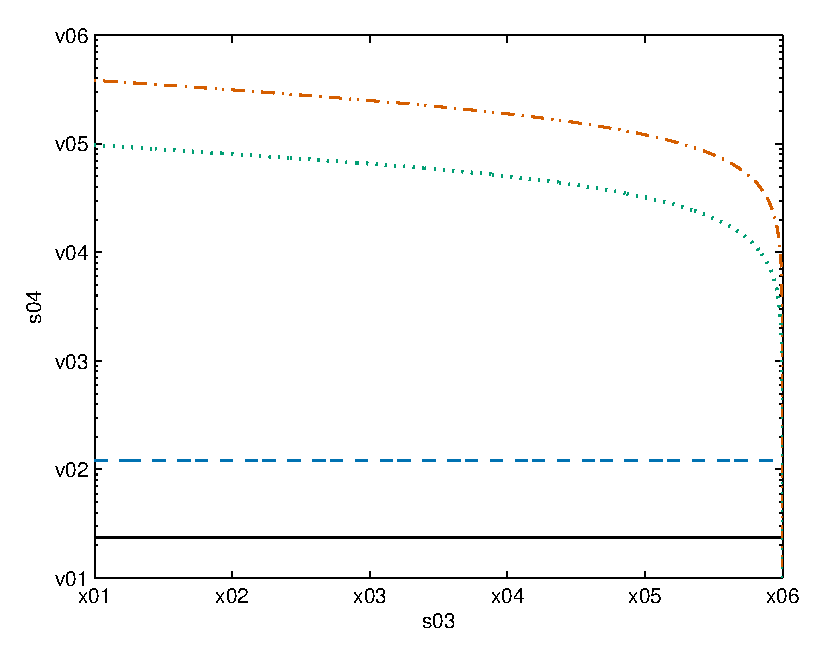
\includegraphics[width=0.45\textwidth]{Inner_cut_1.eps}} \quad 
   \subfigure[{White dwarfs}]{\includegraphics[width=0.45\textwidth]{Inner_cut_2.eps}} \\
   \subfigure[{Neutron stars}]{\includegraphics[width=0.45\textwidth]{Inner_cut_3.eps}} \quad
   \subfigure[{Black holes}]{\includegraphics[width=0.45\textwidth]{Inner_cut_4.eps}}
\caption{Inner cut-off radii for the Galactic Centre as a function of eccentricity. The solid line is the Schwarzschild radius of the MBH; the dashed line is the tidal radius; the dot-dashed line is the collisional cut-off, and the dotted line is the transition to the GW-dominated inspiral regime.\label{fig:Cuts}}
  \end{center}
\end{figure*}

\subsubsection{Tidal disruption}

Tidal forces from the MBH can disrupt stars. This occurs at the tidal radius
\begin{equation}
r\sub{T} \simeq \left(\frac{M_\bullet}{M}\right)^{1/3}R_M
\label{eq:Tidal}
\end{equation}
where $R_M$ is the radius of the star \citep{Hills1975, Rees1988, Kobayashi2004}.\footnote{See \citet{Kesden2012} for a general relativistic treatment.} Any star on an orbit with $r\sub{p} < r\sub{T}$ is disrupted in the course of its orbit. Parametrising orbits by their periapsis allows us to easily determine which stars should be disrupted. We do not include the full effects of the loss cone \citep{Frank1976, Lightman1977, Cohn1978} as these were not incorporated into the Fokker-Planck calculations \citep{Hopman2009}.\footnote{The loss cone is a region in velocity space where orbits are depleted because stars are disrupted more rapidly than they can be replenished by two-body scattering.} The effect of the loss cone should be small, only modifying the DF by a logarithmic term \citep{Lightman1977, Bahcall1977, Cohn1978}. Its effects are diluted by resonant relaxation \citep{Hopman2007,Toonen2009,Merritt2011}. Furthermore, the loss cone could be refilled by the wandering of the MBH because of perturbations from the inhomogeneities in the stellar potential \citep{Sigurdsson1997,Chatterjee2002,Merritt2007}.

Tidal disruption is significant for MS stars since they are least dense: calculated in this way, only MS stars would be tidally disrupted outside of the MBH's event horizon \citep{Sigurdsson1997}. The tidal radius defines the cut-off for periapsis of high eccentricity ($e \ga 1$) orbits \citep{Lightman1977}.

\subsubsection{Relaxation time-scale}\label{sec:Relax}

The motion of a star is determined not only by the dominant influence of the central MBH, but also by the other stars. The gravitational potential of the stars may be split into two components: a smooth background representing the average distribution of stars, and statistical fluctuations from random deviations in the stellar distribution. The former only contributes to the stars' orbits: we neglect this since we are more interested in the influence of the MBH. The latter may be approximated as a series of two-body encounters. These lead to scattering, in a manner much like Brownian motion \citep{Bekenstein1992,Maoz1993,Nelson1999}.

The two-body interactions mostly lead to small deflections. Over time, these may accumulate into a significant change in the dynamics. The relaxation time-scale characterises the time taken for this to happen \citep[section 1.2.1]{Binney2008}. It therefore quantifies the time over which an orbit may be repopulated by scattering. There are a variety of definitions for the relaxation time-scale. For a system with a purely Maxwellian distribution, the time-scale has form
\begin{equation}
\tau\sub{R}\super{Max} \simeq \kappa\frac{\sigma^3}{G^2M_\star^2 n_\star\ln\Lambda},
\label{eq:tauMaxwell}
\end{equation}
where the Coulomb logarithm is $\ln\Lambda = \ln(M_\bullet/M_\star)$ \citep{Bahcall1976}, and $\kappa$ is a dimensionless number. In his pioneering work, \citet{Chandrasekhar1941, Chandrasekhar1960} defined the time-scale as the period over which the squared change in energy was equal to the kinetic energy squared, this gives $\kappa = 9/16\sqrt{\pi} \simeq 0.32$. Subsequently, \citet{Chandrasekhar1941a} described relaxation statistically, treating fluctuations in the gravitational field probabilistically; this gives $\kappa = 9/2(2\pi)^{3/2} \simeq 0.29$. \citet{Bahcall1977} define a reference time-scale from their Boltzmann equation with $\kappa = 3/4\sqrt{8\pi} \simeq 0.15$; this is equal to the reference time-scale defined as the reciprocal of the coefficient of dynamical friction by \citet{Chandrasekhar1943a, Chandrasekhar1943}. \citet{Spitzer1958} define a reference time-scale from the gravitational Boltzmann equation of \citet{Spitzer1951} where $\kappa = \sqrt{2}/\pi \simeq 0.45$. Following \citet{Spitzer1971}, \citet[section 7.4.5]{Binney2008} estimate the time-scale from the velocity diffusion coefficient of the Fokker-Planck equation yielding $\kappa \simeq 0.34$.

All these approaches yield consistent values, suggesting, as a first approximation, any should be valid. We will follow the classic treatment of \citet[chapter 2]{Chandrasekhar1960} which is transparent in its assumptions, adapting from a Maxwellian distribution of velocities to one derived from the DFs \eqnref{Unbound_DF} and \eqnref{Bound_DF}. This, at least, makes the model self-consistent. Since there is uncertainty in the astrophysical parameters, we will not be concerned by small discrepancies in the numerical prefactor that result from the simplifying approximations of this approach. The derivation of the relaxation time-scale along with a discussion of its short-comings are included in \apref{time-scale}. An average time-scale for the entire system is defined in \eqnref{system-relax}, and an average for an orbit is defined in \eqnref{orbital-relax}. We defer any investigation of the consequences of using an alternative formulation for future work, as differences may well be negligible whilst the computation can be complicated.

Two-body interactions lead to diffusion in both energy and angular momentum. When considering a single (bound) orbit, over a relaxation time-scale the energy changes by order of itself while the angular momentum changes by the angular momentum of a circular orbit with that energy $\mathcal{J}\sub{circ}(\mathcal{E})$ \citep{Lightman1977, Rauch1996, Hopman2005}:\footnote{The circular-orbit angular momentum is the maximum value for orbits of that energy.}
\begin{equation}
\left(\frac{\Delta\mathcal{E}}{\mathcal{E}}\right)^{2} \approx \left[\frac{\Delta \mathcal{J}}{\mathcal{J}\sub{circ}(\mathcal{E})}\right]^{2} \approx \frac{t}{\tau\sub{R}}.
\label{eq:diffuse-relax}
\end{equation}
We may define another angular momentum relaxation time-scale as the time taken for the angular momentum to change by order of itself \citep{Merritt2011}
\begin{align}
\tau_\mathcal{J} = {} & \left[\frac{\mathcal{J}}{\mathcal{J}\sub{max}(\mathcal{E})}\right]^2\tau\sub{R} \\
 = {} & \left(1 - e^2\right) \tau\sub{R}.
\label{eq:J-time}
\end{align}
This can be much shorter than the energy relaxation time-scale: diffusion in angular momentum can proceed more rapidly than diffusion in energy.

\subsubsection{Gravitational wave inspiral}\label{sec:GW-in}

Stars orbiting about the MBH continually emit gravitational radiation; this carries away energy and angular momentum, causing the stars to inspiral. Using the analysis of \citet{Peters1963} and \citet{Peters1964} for Keplerian binaries it is possible to define a characteristic inspiral time-scale from the rate of change of energy. For consistency with the definition of the relaxation time-scale, we define the characteristic inspiral time-scale as \citep{MiraldaEscude2000, Merritt2011}
\begin{equation}
\tau\sub{GW} \simeq \mathcal{E}\left\langle\diff{\mathcal{E}}{t}\right\rangle^{-1},
\label{eq:tGW-def}
\end{equation}
where the term in angular brackets is the orbit-averaged rate of energy radiation. Using \eqnref{Energy_ecc} and equation (16) of \citet{Peters1963}
\begin{align}
\tau\sub{GW} \simeq {} & \frac{5}{64}\frac{c^5r\sub{p}^4}{G^3MM_\bullet\left(M + M_\bullet\right)}\frac{(1+e)^{7/2}}{(1-e)^{1/2}} \nonumber \\*
 {} & \times {} \left(1+\frac{73}{24}e^2 + \frac{37}{96}e^4\right)^{-1} \\
 \approx {} & \frac{5}{64}\frac{c^5r\sub{p}^4}{G^3MM_\bullet^2}\frac{(1+e)^{7/2}}{(1-e)^{1/2}}\left(1+\frac{73}{24}e^2 + \frac{37}{96}e^4\right)^{-1}.
\end{align}
For comparison, the total time taken for the inspiral, if undisturbed, is given in \eqnref{Bound_inspiral}. The characteristic time-scale is a better measure of the depletion of an orbit as it only depends upon the parameters of that orbit, and not its future evolution.

The time-scale associated with changes in angular momentum is \citep{Peters1964}
\begin{align}
\tau_{\mathrm{GW},\, \mathcal{J}} \simeq {} & \mathcal{J}\left\langle\diff{\mathcal{J}}{t}\right\rangle^{-1} \\
 \simeq {} & \frac{5}{32}\frac{c^5r\sub{p}^4}{G^3MM_\bullet\left(M + M_\bullet\right)}\frac{(1+e)^{5/2}}{(1-e)^{3/2}}\left(1+\frac{7}{8}e^2\right)^{-1} \\
 \approx {} & \frac{5}{32}\frac{c^5r\sub{p}^4}{G^3MM_\bullet^2}\frac{(1+e)^{5/2}}{(1-e)^{3/2}}\left(1+\frac{7}{8}e^2\right)^{-1}.
\end{align}
This is always greater than the energy time-scale; hence, we only consider changes in energy from gravitational wave emission as important for evolution of the system \citep{Hopman2005}.

Unbound stars only undergo a single periapse passage and only radiate one burst of radiation; we therefore neglect any evolution in their orbital parameters.\footnote{Using the analysis of \citet{Turner1977} it is possible to show that the relative changes in eccentricity $\Delta e / e$ and periapsis $\Delta r\sub{p} / r\sub{p}$ for an extreme mass-ratio binary are less than $\sqrt{e}\,\order{\eta}$, where $\eta = M/M_\bullet$ is small, and so are only important for very high eccentricity orbits (\apref{Unbound}). These are very high energy, and exponentially rare because of the Boltzmann factor in \eqnref{Unbound_DF}.}

The $(1-e)^{-1/2}$ dependence of $\tau\sub{GW}$ for bound orbits connects the two regimes. The rate of change of energy goes to zero as a consequence of the assumption that the orbital parameters do not change over the course of a single orbit. This was necessary to calculate the orbit-averaged quantity. It is a valid approximation since the large mass-ratio ensures a slow evolution of the system (\apref{Unbound}).

When comparing with the relaxation time-scale we are in effect comparing rates of change, with the shorter time-scale highlighting the more rapid process that will dominate the evolution \citep{Amaro-Seoane2007}. We shall therefore compare $\tau\sub{GW}$ with the orbital relaxation time-scale $\tau_\mathcal{J}$ \citep{Merritt2011}. Orbits with inspiral time-scales shorter than orbital relaxation time-scales become depleted by gravitational wave emission faster than they are replenished by scattering. The cusp will not extend to these orbits. Yet, these orbits are not totally depopulated as an object may pass through during its inspiral from a greater periapse and eccentricity. The net effect is that the distributions of MS stars, WDs and NSs are relatively unchanged from their cusp states, but the BH population is significantly depleted.

\subsubsection{Collisions}\label{sec:Collision}

As a consequence of the higher densities in the galactic core, stars may undergo a large number of close encounters with other stars \citep{Cohn1978}. These may lead to their destruction. MS stars, WDs, and NSs may be pulled apart by tidal forces if they stray too close to a a more massive object. As MS stars are diffuse, they would not tidally disrupt another star \citep{Murphy1991,Freitag2005}, close encounters would result in some mass transfer; however, the cumulative effect of $20$--$30$ grazing collisions could disrupt a MS star \citep{Freitag2006}. The number of collisions a star shall undergo in a time interval $\delta t$ is
\begin{equation}
\delta K = n(r) A v(r,e,r\sub{p})\delta t,
\end{equation}
where $A$ is the collisional cross-sectional area. For tidal disruption, where the encounter is with a collapsed object (WD, NS or BH), we set $A = \pi r_{\mathrm{T},\,{M'}}^2$, where $r_{\mathrm{T},\,{M'}}$ is the appropriate tidal radius: it is the same as \eqnref{Tidal} but with $M_\bullet$ replaced with the mass of the collapsed object $M'$. For collisions between MS stars, the cross-sectional area is simply the geometric $A = \pi R_\star^2$.\footnote{Here we assume that the relative velocity of the colliding stars is much greater than the escape velocity of the star so we may neglect the effects of gravitational focusing.}

For circular orbits we can find the radius at which collisions lead to disruptions by setting $\delta K = 1$ for tidal disruption or $\delta K = 20$ for grazing collisions, and $\delta t = \tau\sub{R}$. We use the relaxation time-scale for the system as this is the time over which stars are replenished from the reservoir. For non-circular orbits we must consider variation with position. Using $\delta r = v_r \delta t$, and then converting to an integral, we have for bound orbits
\begin{equation}
K = 2 A \frac{\tau\sub{R}}{P(r\sub{p},e)}\intd{r\sub{p}}{(1+e)r\sub{p}/(1-e)}{n(r)\frac{v(r,e,r\sub{p})}{v_r(r,e,r\sub{p})}}{r},
\end{equation}
where $P$ is the period of the orbit. Again we may set $K = 1$ or $K = 20$ to find the orbits for which stars will be disrupted within a relaxation time-scale (of the system). For unbound orbits we are only interested in stars that would become disrupted before their periapse passage, so
\begin{equation}
K = A \intd{r\sub{p}}{r\sub{c}}{n(r)\frac{v(r,e,r\sub{p})}{v_r(r,e,r\sub{p})}}{r},
\end{equation}
assuming that the stars in the reservoir external to the core are unlikely to undergo close collisions.

Collisions provide the cutoff for MS stars, and are significant for WDs.


\section*{Acknowledgments}
The authors are grateful for insightful discussions with Sverre Aarseth. The authors thank Tal Alexander and Clovis Hopman for useful correspondence. CPLB is supported by STFC. JRG is supported by the Royal Society.

\bibliographystyle{mn3e}
\bibliography{Galactic}

\appendix

\begin{onecolumn}

\section{Chandrasekhar's relaxation time-scale}\label{sec:time-scale}

\citet[chapter 2]{Chandrasekhar1960} defined a relaxation time-scale for a stellar system by approximating the fluctuations in the stellar gravitational potential as a series of two-body encounters. The time over which the squared change in energy is equal to the (initial) kinetic energy of the star is the time taken for relaxation. Relaxation is explained through dynamical friction (\citealt{Chandrasekhar1943a}; \citealt[section 1.2]{Binney2008}). This can be understood intuitively as the drag induced on a star by the over-density of field stars deflected by its passage \citep{Mulder1983}. In the interaction between the star and its gravitational wake, energy and momentum are exchanged, accelerating some stars, decelerating others.

Chandrasekhar's approach has proved exceedingly successful despite the number of simplifying assumptions inherent in the model which are not strictly applicable to systems such as the Galactic centre. We will not attempt to fix these deficiencies, rather, the only modification to the standard picture shall be to substitute the velocity distribution: while the canonical formulation uses a simple homogeneous Gaussian distribution, we use a distribution derived from the distribution functions \eqnref{Unbound_DF} and \eqnref{Bound_DF}.

Other authors have built upon the work of Chandrasekhar by considering inhomogeneous stellar distributions, via perturbation theory \citep{Lynden-Bell1972,Tremaine1984,Weinberg1986}; modelling energy transfer as anomalous dispersion, which adds higher order moments to the transfer probability \citep{Bar-Or2012}, or using the tools of linear response theory and the fluctuation-dissipation theory \citep[chapter 7]{Landau1958}, which allows relaxation of certain assumptions, such as homogeneity \citep{Bekenstein1992,Maoz1993,Nelson1999}. We will not attempt to employ such sophisticated techniques at this stage.

\subsection{Chandrasekhar's derivation of the change in energy}\label{sec:Chandra}

We consider the interaction of a field star, denoted by 1, with a test star, 2; the centre-of-gravity and relative velocities are
\begin{subequations}
\begin{align}
\boldsymbol{V}\sub{g} = {} & \recip{m_1 + m_2}\left(m_1 \boldsymbol{v}_1 + m_2 \boldsymbol{v}_2\right);\\
\boldsymbol{V} = {} & \boldsymbol{v}_1 - \boldsymbol{v}_2.
\end{align}
\label{eq:Vs}
\end{subequations}
Hence
\begin{subequations}
\begin{align}
v_1^2 = {} & V\sub{g}^2 - 2\frac{m_2}{m_1 + m_2}V\sub{g}V \cos\Phi + \left(\frac{m_2}{m_1 + m_2}\right)^2V^2;\\
v_2^2 = {} & V\sub{g}^2 + 2\frac{m_1}{m_1 + m_2}V\sub{g}V \cos\Phi + \left(\frac{m_1}{m_1 + m_2}\right)^2V^2,
\end{align}
\end{subequations}
where $\Phi$ is the angle between $\boldsymbol{V}\sub{g}$ and $\boldsymbol{V}$, and
\begin{subequations}
\begin{align}
V\sub{g}^2 = {} & \recip{(m_1 + m_2)^2}\left(m_1v_1^2 + m_2v_2^2 + 2 m_1 m_2 v_1 v_2 \cos\theta\right);\\
V^2 = {} & v_1^2 + v_2 - 2 v_1 v_2 \cos\theta,
\end{align}
\label{eq:V2s}
\end{subequations}
where $\theta$ is the angle between $\boldsymbol{v}_1$ and $\boldsymbol{v}_2$. The change in energy of during the interaction is
\begin{align}
\Delta E = {} & \recip{2} m_2 \left({v'_2}^2 - v_2^2\right)\\
 = {} & \frac{m_1 m_2}{m_1 + m_2}V\sub{g}V\left(\cos\Phi' - \cos\Phi\right),
\end{align}
using primed variables for values after the interaction, and unprimed ones for before. If we project the angle out onto the orbital plane
\begin{equation}
\Delta E = \frac{m_1 m_2}{m_1 + m_2}V\sub{g}V\left(\cos\phi' - \cos\phi\right)\cos i,
\end{equation}
where $\phi$ is the angle in the plane, and $i$ is the inclination of $\boldsymbol{V}\sub{g}$ out of the plane. We define the deflection angle $\psi$ such that
\begin{equation}
\phi' - \phi = \pi - 2\psi,
\end{equation}
hence
\begin{equation}
\Delta E = -2\frac{m_1 m_2}{m_1 + m_2}V\sub{g}V\cos(\phi - \psi)\cos\psi\cos i.
\end{equation}

We now need to calculate the encounter rate. This requires us to know number of field stars per unit volume and per volume space element. We make the simplifying assumption that the density of stars is uniform. This is not the case for the Galactic centre; however, we approximate it as so in order to make the problem tractable. It may seem especially bad for treatment of compact objects very close to the central MBH, inside the radius where main sequence stars would be tidally disrupted; however, it must be remembered that it is small angle deflections, rather than large deflections from close collisions, that are most important for relaxation. The error introduced by this assumption can be partially absorbed by the appropriate choice of the Coloumb logarithm, which shall be introduced later~\citep{Just2011}. Using an averaged value, the number of stars is
\begin{equation}
\dd N = n(v_1, \theta, \varphi)\,\dd v_1 \,\dd \theta \,\dd \varphi \,\dd^3r,
\end{equation}
using spherical polar coordinates for velocity space. Using $D$ as the impact parameter for the encounter and $\Theta$ for the angle between the fundamental plane (containing $\boldsymbol{v}_1$ ans $\boldsymbol{v}_2$) and the the orbital plane, the number of events in time interval $\delta t$ is
\begin{equation}
\dd \Gamma =  n(v_1, \theta, \varphi)\,\dd v_1 \,\dd \theta \,\dd \varphi \frac{\dd \Theta}{2\pi} 2\pi D \,\dd D V \,\delta t.
\end{equation}
The squared change in energy for these encounters is
\begin{align}
\Delta E^2(v_1,\theta,\varphi,D,\Theta) = {} & \left(\Delta E\right)^2\,\dd \Gamma\\
 = {} & 4 n(v_1,\theta,\varphi)V\sub{g}^2V^3\left(\frac{m_1m_2}{m_1+m_2}\right)^2\cos^2i\cos^2(\phi-\psi)\cos^2\psi D\,\dd v_1\,\dd\theta\,\dd\varphi\,\dd\Theta\,\dd D\,\delta t.
\end{align}
We must integrate out all these dependencies.

Since we have assumed that the stellar density does not depend upon position, we can simply integrate over the impact parameter; this is related to the deflection angle by
\begin{equation}
\recip{\cos^2\psi} = 1 + \frac{D^2V^4}{G(m_1 + m_2)}.
\end{equation}
Thus
\begin{equation}
\Delta E^2(v_1,\theta,\varphi,\psi,\Theta) =  4 n(v_1,\theta,\varphi)\frac{V\sub{g}^2}{V}G^2m_1^2 m_2^2\cos^2i\frac{\cos^2(\phi-\psi)\sin\psi}{\cos\psi} \,\dd \psi\,\dd v_1\,\dd\theta\,\dd\varphi\,\dd\Theta\,\delta t.
\end{equation}
The integral over $\psi$ is
\begin{align}
I(\psi_0) = {} & \intd{0}{\psi_0}{\frac{\cos^2(\phi-\psi)\sin\psi}{\cos\psi}}{\psi}\\
 = {} & \frac{\sin 2\phi}{2}\left(\psi_0 - \frac{\sin 2\psi_0}{2}\right) - \frac{\cos 2\phi}{2}\left(\frac{\cos 2\psi_0}{2}\right) - \sin^2\phi\ln(\cos\psi_0).
\end{align}
Naively we would think that the upper limit for the deflection limit should be $\psi_0 = \pi/2$; however, this would introduce a logarithmic divergence. In actuality there is a physical cut-off, reflecting a finite bound for the maximum impact parameter $D_0$ \citep{Weinberg1986}. This is set by the scale of the system, beyond which scattering is negligible. While the logarithmic term is finite, it is still large, dominating the other terms which are $\order{1}$; we therefore neglect the subdominant terms
\begin{equation}
\Delta E^2(v_1,\theta,\varphi,\Theta) \simeq  4 n(v_1,\theta,\varphi)\frac{V\sub{g}^2}{V}G^2m_1^2 m_2^2\cos^2i\sin^2\phi\ln\left(\recip{\cos\psi_0}\right)\,\dd v_1\,\dd\theta\,\dd\varphi\,\dd\Theta\,\delta t.
\end{equation}

Next, we integrate over the orbital plane inclination using
\begin{equation}
\cos i\sin\phi = \sin\Phi\cos\Theta,
\end{equation}
so that
\begin{equation}
\Delta E^2(v_1,\theta,\varphi) \simeq  4\pi n(v_1,\theta,\varphi)\frac{V\sub{g}^2}{V}G^2m_1^2 m_2^2\sin^2\Phi\ln\left(\recip{\cos\psi_0}\right)\,\dd v_1\,\dd\theta\,\dd\varphi\,\delta t.
\end{equation}
We are now left with just the velocity variables.

An expression for $\sin^2\Phi$ can be obtained from \eqnref{Vs} and \eqnref{V2s}, after some rearrangement
\begin{equation}
\frac{V_g^2}{V}\sin^2\Phi = \frac{v_1^2v_2^2\sin^2\theta}{\left(v_1^2 + v_2^2 - 2v_1 v_2 \cos\theta\right)^{3/2}}.
\end{equation}
To proceed further we must specify the form of $n(v_1,\theta,\varphi)$, if we assume isotropy
\begin{equation}
n(v_1,\theta,\varphi) = n(v_1)\recip{4\pi}\sin\theta.
\end{equation}
The integral over $\varphi$ is then trivial,
\begin{equation}
\Delta E^2(v_1,\theta) \simeq \pi n(v_1)\frac{G^2m_1^2 m_2^2v_1^2v_2^2\sin^3\theta}{\left(v_1^2 + v_2^2 - 2v_1 v_2 \cos\theta\right)^{3/2}}\ln\left[1 + \frac{D_0\left(v_1^2 + v_2^2 - 2v_1 v_2 \cos\theta\right)^2}{G^2\left(m_1 + m_2\right)^2}\right]\,\dd v_1\,\dd\theta\,\delta t.
\end{equation}

To integrate over $\theta$ it is easier to recast in terms of $V$; the integral is
\begin{align}
J = {} & v_1^2 v_2^2 \intd{0}{\pi}{\frac{\sin^3\theta}{\left(v_1^2 + v_2^2 - 2v_1 v_2 \cos\theta\right)^{3/2}}\ln\left[1 + \frac{D_0\left(v_1^2 + v_2^2 - 2v_1 v_2 \cos\theta\right)^2}{G^2\left(m_1 + m_2\right)^2}\right]}{\theta} \\
 = {} & v_1 v_2 \intd{V_-}{V_+}{\frac{\sin^2\theta}{V^2}\ln\left(1 + q^2V^4\right)}{V},
\end{align}
where the limits are
\begin{equation}
V_+ = v_1 + v_2; \quad V_- = |v_1 - v_2|,
\end{equation}
and we have introduced
\begin{equation}
q = \frac{D_0}{G\left(m_1+m_2\right)}.
\end{equation}
Using \eqnref{V2s} to rearrange, and then integrating by parts gives
\begin{align}
J = {} & \recip{4 v_1 v_2} \intd{V_-}{V_+}{\frac{\left(V_+^2 - V^2\right)\left(V^2 - V_-^2\right)}{V^2}\ln\left(1 + q^2V^4\right)}{V} \\
 = {} & \recip{4 v_1 v_2} \left\{\left[\frac{3V_+^2V_-^2 + 3\left(V_+^2 + V_-^2\right)V^2 - V^4}{3V} \ln\left(1 + q^2V^4\right)\right]^{V_+}_{V_-} - \intd{V_-}{V_+}{\frac{3V_+^2V_-^2 + 3\left(V_+^2 + V_-^2\right)V^2 - V^4}{3V}\frac{4q^2V^3}{1+ q^2V^4}}{V}\right\};
\end{align}
the former piece still contains the logarithmic term which we know must be large. It is therefore the dominant piece of the integral and we neglect the latter \citep{Chandrasekhar1941},
\begin{equation}
J \simeq \recip{6 v_1 v_2} \left[\left(3V_-^2 + V_+^2\right)V_+\ln\left(1 + q^2V_+^4\right) - \left(3V_+^2 + V_-^2\right)V_-\ln\left(1 + q^2V_-^4\right)\right].
\end{equation}
This may be further simplified, reusing the limit of large $q$ \citep{Chandrasekhar1941,Chandrasekhar1941b},
\begin{align}
J \simeq {} & \recip{3 v_1 v_2} \left[\left(3V_-^2 + V_+^2\right)V_+\ln\left(qV_+^2\right) - \left(3V_+^2 + V_-^2\right)V_-\ln\left(qV_-^2\right)\right] \\
 \simeq {} & \frac{4}{3v_1v_2}\begin{cases}
\left(v_1^3 + v_2^3\right)\ln\left[q\left(v_1 + v_2\right)^2\right] - \left(v_2^3 - v_1^3\right)\ln\left[q\left(v_1 - v_2\right)^2\right] & v_1 \leq v_2 \\
\left(v_1^3 + v_2^3\right)\ln\left[q\left(v_1 + v_2\right)^2\right] - \left(v_1^3 - v_2^3\right)\ln\left[q\left(v_1 - v_2\right)^2\right] & v_1 \geq v_2
\end{cases} \\
 \simeq {} & \frac{8}{3}\begin{cases}
\dfrac{v_2^2}{v_1}\ln\left(\dfrac{v_1 + v_2}{v_2 - v_1}\right) + \dfrac{v_1^2}{v_2}\left[\ln\left(qv_2^2\right) + \ln\left(1 - \dfrac{v_1^2}{v_2^2}\right)\right] & v_1 < v_2 \\
v_2\left[\ln\left(qv_2^2\right) + \ln 4\right] & v_1 = v_2\\
\dfrac{v_1^2}{v_2}\ln\left(\dfrac{v_1 + v_2}{v_1 - v_2}\right) + \dfrac{v_2^2}{v_1}\left[\ln\left(qv_2^2\right) + \ln\left(\dfrac{v_1^2}{v_2^2} - 1\right)\right] & v_1 > v_2
\end{cases} \\
\approx {} & \frac{8}{3}\begin{cases}
\dfrac{v_1^2}{v_2}\ln\left(qv_2^2\right) & v_1 \leq v_2 \\
\dfrac{v_2^2}{v_1}\ln\left(qv_2^2\right) & v_1 \geq v_2
\end{cases}.
\end{align}
This form maintains the correct limit for $v_2 \rightarrow 0$. We are left with
\begin{equation}
\Delta E^2(v_1) \simeq \frac{8\pi}{3} n(v_1)G^2m_1^2 m_2^2\ln\left(qv_2^2\right)\left\{\begin{array}{lr}\dfrac{v_1^2}{v_2} & v_1 \leq v_2\\ \dfrac{v_2^2}{v_1} & v_1 \geq v_2 \end{array}\right\}\,\dd v_1\delta t.
\end{equation}
The final integral requires a specific form for the velocity distribution.

\subsection{Velocity distributions}

The velocity space distribution function can be obtained by integrating out the spatial dependence in the full DF
\begin{equation}
f(v) = \int \dd^3r f(\mathcal{E}).
\end{equation}
As we are restricting our attention to the Galactic centre and assuming spherical symmetry
\begin{equation}
f(v) = 4\pi\intd{0}{r\sub{c}}{r^2f(\mathcal{E})}{r},
\end{equation}
where $r_c$ is defined by \eqnref{r_c}. It is useful to work in terms of dimensionless variables
\begin{align}
x = {} & \frac{\mathcal{E}}{\sigma^2}; \\
w = {} & \frac{v^2}{2\sigma^2}.
\end{align}
Changing the integral to be over dimensionless energy
\begin{equation}
f(v) = 4\pi r\sub{c}^3\intd{\infty}{w - 1}{\frac{f(x)}{(w-x)^4}}{x},
\end{equation}
keeping $w$ as a function of $v$.

The DF for unbound stars is assumed to be Maxwellian; it is defined in \eqnref{Unbound_DF} and is applicable for $x > 0$, implying $w > 1$:
\begin{align}
f_{\mathrm{u},\,M}(v) = {} & \frac{N_\ast}{\left(2\pi\sigma^2\right)^{3/2}}C_M \intd{0}{w-1}{\frac{\exp(-x)}{(w-x)^4}}{x} \\
 = {} & \frac{N_\ast}{\left(2\pi\sigma^2\right)^{3/2}}C_M\epsilon\left(\frac{v^2}{2\sigma^2}\right),
\end{align}
introducing
\begin{equation}
\epsilon(w) = \recip{2}\left\{\exp(-w)\left[4\exp(1) + \Ei(w) - \Ei(1)\right] - \frac{2 + w + w^2}{w^3}\right\},
\end{equation}
where $\Ei(x)$ is the exponential integral.

The DF for bound stars is approximated as a simple power law as defined in \eqnref{Bound_DF}, it is applicable for $x < 0$:
\begin{equation}
f_{\mathrm{b},\,M}(v) = \frac{N_\ast}{\left(2\pi\sigma^2\right)^{3/2}}k_M\begin{cases}
\intd{-\infty}{w-1}{\dfrac{(-x)^{p_M}}{(w-x)^4}}{x} & w \leq 1 \\
\intd{-\infty}{0}{\dfrac{(-x)^{p_M}}{(w-x)^4}}{x} & w \geq 1
\end{cases}.
\end{equation}
The integral may be evaluated in terms of the hypergeometric function ${_2F_1(a,b;c;x)}$, but for the limits needed here the results simplify to
\begin{equation}
f_{\mathrm{b},\,M}(v) = \frac{N_\ast}{\left(2\pi\sigma^2\right)^{3/2}}k_M \left(\frac{v^2}{2\sigma^2}\right)^{p_M - 3}\begin{cases}
3 \Beta\left(\dfrac{v^2}{2\sigma^2}; 3 - p_M, 1 + p_M\right) & \dfrac{v^2}{2\sigma^2} \leq 1 \\
3 \Beta\left(3 - p_M, 1 + p_M\right) & \dfrac{v^2}{2\sigma^2} \geq 1
\end{cases},
\end{equation}
where $\Beta(x;a,b)$ is the incomplete beta function \citep[8.17]{Olver2010}, $\Beta(a,b) \equiv \Beta(1,a,b)$ is the complete beta function.

The velocity space density is related to the distribution by
\begin{equation}
\frac{4\pi r\sub{c}^3}{3}n_M(v_1) = 4\pi v_1^2\left[f_{\mathrm{u},\,M}(v_1) + f_{\mathrm{b},\,M}(v_1)\right].
\end{equation}

\subsection{Defining the relaxation time-scale}

Using the specific forms for the velocity space density, we can calculate the squared change in energy. The functional form depends upon the velocity of the test star. If $v_2^2/2\sigma^2 < 1$, then
\begin{align}
\Delta E^2 \simeq {} & \frac{8}{3}\sqrt{2\pi}\frac{G^2m_1^2 m_2^2n_\ast}{\sigma^3}\ln\left(qv_2^2\right)\left\{\intd{0}{v_2}{3k\frac{v_1^4}{v_2}\left(\frac{v_1^2}{2\sigma^2}\right)^{p-3} \Beta\left(\frac{v_1^2}{2\sigma^2};3 - p, 1 + p\right)}{v_1} \right. \nonumber\\*
 & + \left. \intd{v_2}{\sqrt{2}\sigma}{3kv_1v_2^2\left(\frac{v_1^2}{2\sigma^2}\right)^{p-3} \Beta\left(\frac{v_1^2}{2\sigma^2};3 - p, 1 + p\right)}{v_1} \right. \nonumber\\*
 & + \left. \intd{\sqrt{2}\sigma}{\infty}{v_1v_2^2\left[3 k\left(\frac{v_1^2}{2\sigma^2}\right)^{p-3}\Beta\left(3 - p_M, 1 + p_M\right) + C\epsilon\left(\frac{v_1^2}{2\sigma^2}\right)\right]}{v_1}\right\}\,\delta t,
\end{align}
where we have suppressed the subscript $M$ for brevity; it would be necessary to sum over all the species to get the total value. Computing the integrals and rearranging yields
\begin{align}
\Delta E^2 \simeq {} & \frac{16}{3}\sqrt{2\pi}\frac{G^2m_1^2 m_2^2n_\ast}{\sigma^3}\ln\left(qv_2^2\right) \left(\frac{v_2^2}{2\sigma^2}\right) \left[k \frac{3}{(2 - p)(1 + p)}{_3F_2}\left(-1-p,2-p,\frac{3}{2};3-p,\frac{5}{2};\frac{v_2^2}{2\sigma^2}\right) + C\right]\,\delta t,
\end{align}
where ${_3F_2}(a_1,a_2,a_3;b_1,b_2;x)$ is a generalised hypergeometric function \citep[section 16]{Olver2010}. The contribution from bound and unbound stars can be identified by the coefficients $k$ and $C$ respectively.

If $v_2^2/2\sigma^2 > 1$,
\begin{align}
\Delta E^2 \simeq {} & \frac{8}{3}\sqrt{2\pi}\frac{G^2m_1^2 m_2^2n_\ast}{\sigma^3}\ln\left(qv_2^2\right)\left\{\intd{0}{\sqrt{2}\sigma}{3k\frac{v_1^4}{v_2}\left(\frac{v_1^2}{2\sigma^2}\right)^{p-3} \Beta\left(\frac{v_1^2}{2\sigma^2};3 - p, 1 + p\right)}{v_1} \right. \nonumber\\*
 & + \left. \intd{\sqrt{2}\sigma}{v_2}{\frac{v_1^4}{v_2}\left[3k\left(\frac{v_1^2}{2\sigma^2}\right)^{p-3}\Beta\left(3 - p, 1 + p\right) + C \epsilon\left(\frac{v_1^2}{2\sigma^2}\right)\right]}{v_1} \right. \nonumber\\*
 & \left. + \intd{v_2}{\infty}{v_1v_2^2\left[3k\left(\frac{v_1^2}{2\sigma^2}\right)^{p-3}\Beta\left(3 - p_M, 1 + p_M\right) + C \epsilon\left(\frac{v_1^2}{2\sigma^2}\right)\right]}{v_1}\right\}\,\delta t.
\end{align}
Computing this gives
\begin{equation}
\Delta E^2 \simeq \frac{16}{3}\sqrt{2\pi}G^2m_1^2 m_2^2n_\ast\sigma\ln\left(qv_2^2\right) \left(\frac{v_2^2}{2\sigma^2}\right)^{-1/2} \left[k\beta\left(\frac{v_2^2}{2\sigma^2};p\right) + C\alpha\left(\frac{v_2^2}{2\sigma^2}\right)\right]\,\delta t,
\end{equation}
where
\begin{align}
\alpha(w) = {} & \recip{2}\left\{3w^{-1/2} + 5 + \left[4\exp(1) - \Ei(1) + \Ei(w)\right]\left[\frac{3\sqrt{\pi}}{4}\erf\left(w^{1/2}\right) - \frac{3}{2}w^{1/2}\exp(-w)\right] - 3\sqrt{\pi}\exp(1)\erf(1) \right. \nonumber\\*
 & + \left. 3\left[{_2F_2}\left(\frac{1}{2},1;\frac{3}{2},\frac{3}{2};1\right) - w^{1/2}{_2F_2}\left(\frac{1}{2},1;\frac{3}{2},\frac{3}{2};w\right)\right]\right\}; \\
\beta(w;p) = {} & \begin{cases} \dfrac{3}{1/2 - p}\left[\Beta\left(\dfrac{5}{2},1+p\right) - \dfrac{3w^{p-1/2}}{2(2-p)}\Beta\left(3-p,1+p\right)\right] & p < \recip{2} \\
\dfrac{\pi}{32}\left[12 \ln(2) - 1 + 6 \ln(w)\right] & p = \recip{2} \end{cases} . 
\end{align}
The generalised hypergeometric function originates from the integral
\begin{equation}
\intd{}{w}{\frac{\exp(w')\erf\left({w'}^{1/2}\right)}{w'}}{w'} = \frac{4w^{1/2}}{\sqrt{\pi}}{_2F_2}\left(\frac{1}{2},1;\frac{3}{2},\frac{3}{2};w\right).
\end{equation}

Combining the two regimes gives some quite complicated expressions. It is possible to simplify these while maintaining reasonable accuracy, for this purpose we separate the contributions from bound and unbound stars. The bound contribution is relatively straightforward for larger $v_2$; for smaller $v_2$ we may use a series expansion in $v_2^2/2\sigma^2 < 1$ to approximate the hypergeometric function:
\begin{align}
\Delta E\sub{b}^2 \approx {} & \frac{16}{3}\sqrt{2\pi}G^2m_1^2m_2^2n_\ast\sigma\ln\left(qv_2^2\right) k \left\{\begin{array}{lr}
\dfrac{3}{(1 + p)(2 - p)}\left(\dfrac{v_2^2}{2\sigma^2}\right) - \dfrac{9}{5(3-p)}\left(\dfrac{v_2^2}{2\sigma^2}\right)^2 + \dfrac{9p}{14(7-p)}\left(\dfrac{v_2^2}{2\sigma^2}\right)^3 & \dfrac{v_2^2}{2\sigma^2} < 1 \\
\left(\dfrac{v_2^2}{2\sigma^2}\right)^{-1/2}\beta\left(\dfrac{v_2^2}{2\sigma^2};p\right) & \dfrac{v_2^2}{2\sigma^2} > 1\end{array}\right\}\,\delta t.
\end{align}
This can be rolled into one continuous function
\begin{align}
\Delta E\sub{b}^2 \approx {} & \frac{16}{3}\sqrt{2\pi}G^2m_1^2m_2^2n_\ast\sigma\ln\left(qv_2^2\right) k \left[1 + \left(\frac{v_2^2}{2\sigma^2}\right)^4\right]^{-1}\left\{\left[\dfrac{3}{(1 + p)(2 - p)}\left(\dfrac{v_2^2}{2\sigma^2}\right) - \dfrac{9}{5(3-p)}\left(\dfrac{v_2^2}{2\sigma^2}\right)^2 + \dfrac{9p}{14(7-p)}\left(\dfrac{v_2^2}{2\sigma^2}\right)^3 \right]\right. \nonumber\\*
 & + \left. \left(\frac{v_2^2}{2\sigma^2}\right)^{7/2}\beta\left(\frac{v_2^2}{2\sigma^2};p\right)\right\}\,\delta t\\
 \approx {} & 16\sqrt{2\pi}G^2m_1^2m_2^2n_\ast\sigma\ln\left(qv_2^2\right) k \gamma\left(\frac{v_2^2}{2\sigma^2};p\right)\,\delta t,
\label{eq:Bound-approx}
\end{align}
defining the function $\gamma(w;p)$ in the last line. The resulting error [ignoring variation from $\ln\left(qv_2^2\right)$] is less than $3\%$.

The unbound contribution is very simple for small $v_2$, but much more complicated for large $v_2$. In the limit of $v_2 \rightarrow \infty$, it decays as $v_2^{-1}$:
\begin{align}
\lim_{w \rightarrow \infty}\left\{\alpha(w)\right\} = {} & \recip{2}\left\{5 + 3\sqrt{\pi}\left[\exp(1) - \frac{\Ei(1)}{4} - \exp(1)\erf(1)\right] + 3{_2F_2}\left(\frac{1}{2},1;\frac{3}{2},\frac{3}{2};1\right)\right\} \\
 = {} & \Xi \simeq 4.31.
\end{align}
Using the two limiting forms, the function
\begin{equation}
\Delta E\sub{u}^2 \approx \frac{16}{3}\sqrt{2\pi}G^2m_1^2m_2^2n_\ast\sigma\ln\left(qv_2^2\right) C \Xi\left(\frac{v_2^2}{2\sigma^2}\right)\left[\Xi^2 + \left(\frac{v_2^2}{2\sigma^2}\right)^3\right]^{-1/2}\,\delta t,
\label{eq:Unbound-approx}
\end{equation}
reproduces the full function to better than $5\%$ [ignoring variation from $\ln\left(qv_2^2\right)$].

Making explicit the sum over the different species, the total change in energy squared is approximately
\begin{equation}
\Delta E^2 \approx \sum_M \frac{16}{3}\sqrt{2\pi}G^2 M^2m_2^2n_\ast\sigma\ln\left(qv_2^2\right) \left\{k_M \gamma\left(\frac{v_2^2}{2\sigma^2};p_M\right) + C_M\Xi\left(\frac{v_2^2}{2\sigma^2}\right)\left[\Xi^2 + \left(\frac{v_2^2}{2\sigma^2}\right)^3\right]^{-1/2}\right\}\,\delta t.
\end{equation}
The relaxation time-scale is the time interval $\delta t$ over which the squared change in energy becomes equal to the kinetic energy of the test star squared \citep{Bar-Or2012}
\begin{align}
\tau\sub{R} = {} & \left(\frac{m_2v_2^2}{2}\right)^2\frac{\delta t}{\Delta E^2} \\
 \approx {} & \frac{3v_2^4}{16\sqrt{2\pi}G^2n_\ast\sigma\ln\left(qv_2^2\right)} \left(\sum_M M^2 \left\{k_M \gamma\left(\frac{v_2^2}{2\sigma^2};p_M\right) + C_M\Xi\left(\frac{v_2^2}{2\sigma^2}\right)\left[\Xi^2 + \left(\frac{v_2^2}{2\sigma^2}\right)^3\right]^{-1/2}\right\}\right)^{-1}.
\end{align}
This is the time required for stellar encounters to become effective in changing the energy of an orbit in the smooth background potential. The use of the squared change in energy reflects the expectation that energy changes like a random walk, and hence scales with the square-root of the time.

\subsection{Averaged time-scale}

The relaxation time-scale defined above is appropriate for a particular initial test star velocity $v_2$. This is not of much use to describe the Galactic centre or even a (non-circular) orbit where there is a range in velocity. It is necessary to calculate an averaged time-scale. Both the change in energy squared and the kinetic energy are averaged; comparing these gives the appropriate time-scale. We shall use two averages: over the distribution of bound velocities to give the relaxation time-scale for the system, and over a single orbit. The former shall be of use when considering the inner cut-off of stars due to collisions, the latter when considering the transition to gravitational wave inspiral.

\subsubsection{System relaxation time-scale}\label{sec:system-ave}

The total number of bound stars in the core is
\begin{equation}
N_{\mathrm{b},\,M} = \frac{3}{3/2 - p_M}\frac{\Gamma(p_M + 1)}{\Gamma(p_M + 7/2)}N_\ast k_M,
\end{equation}
where $\Gamma(x)$ is the gamma function. Using this as a normalisation constant, the probability of a bound star having a velocity in the range $v \rightarrow v + \dd v$ is given by
\begin{align}
4\pi v^2 p_{\mathrm{b},\,M}(v) \,\dd v = {} & 4\pi v^2 \frac{f_{\mathrm{b},\,M}(v)}{N_{\mathrm{b},\,M}} \,\dd v \\
 = {} & \sqrt{\frac{2}{\pi}} \frac{v^2}{\sigma^3} \frac{\left(3/2 - p_M\right)\Gamma(p_M + 7/2)}{\Gamma(p_M + 1)} \left(\frac{v^2}{2\sigma^2}\right)^{p_M - 3}\left\{\begin{array}{lr}
\Beta\left(\dfrac{v^2}{2\sigma^2}; 3 - p_M, 1 + p_M\right) & \dfrac{v^2}{2\sigma^2} \leq 1 \\
\Beta\left(3 - p_M, 1 + p_M\right) & \dfrac{v^2}{2\sigma^2} \geq 1\end{array}\right\}\,\dd v.
\end{align}
The mean squared velocity for bound stars in the core is then
\begin{align}
\overline{v^2_{M}} = {} & 4\pi\intd{0}{\infty}{v^4 p_{\mathrm{b},\,M}(v)}{v} \\
 = {} & 3\sigma^2\frac{3/2 - p_M}{1/2 - p_M},
\end{align}
assuming that $p_M < 1/2$.

In the case $p_M = 1/2$ the integral no longer converges, we encounter a logarithmic divergence. This is not a concern, just as with the divergence encountered in \secref{Chandra}, it reflects there being a physical cut-off; in this case there is a maximal velocity. We use $v\sub{max} = c/2$, which is the maximum speed reached on a bound orbit about a Schwarzschild BH. Marginally higher speeds can be reached for prograde orbits about a Kerr BH, but the maximal velocity for retrograde orbits is marginally lower. In reality, we might expect the maximum velocity to be lower due to a depletion of orbits (for example because of gravitational wave inspiral). We neglect these possible variations, since the error introduced should be small as a consequence of taking the logarithm. We also suspect that a simple Newtonian description of these orbits is imprecise, but a full relativistic description is beyond this simple analysis. For $p_M = 1/2$,
\begin{align}
\overline{v^2_{M}} = {} & \frac{\sigma^2}{2}\left[12\ln(2) - 5 + 6 \ln\left(\frac{v\sub{max}^2}{2\sigma^2}\right)\right].
\end{align}
Using a typical value of $\sigma = 10^5\units{m\,s^{-1}}$,
\begin{equation}
\overline{v^2_{M}} \simeq 43\sigma^2.
\end{equation}
The mean squared velocity is an order of magnitude greater than for a Maxwellian distribution.

The average of the change in energy is more involved. First we replace the term $\ln\left(qv_2^2\right)$ in $\Delta E^2$ by a suitable average so that it may be moved outside the integral \citep[chapter 2]{Chandrasekhar1960}. We assume that it may be replaced by the Coulomb logarithm, which can be approximated as \citep{Bahcall1976}
\begin{equation}
\ln\left(q\overline{v_2^2}\right) = \ln \Lambda_M \simeq \ln\left(\frac{M_\bullet}{M}\right).
\end{equation}
\citet{Just2011} find an extremely similar result fitting a Bahcall--Wolf cusp self-consistently. We calculate the averages for the bound and unbound contributions individually. In calculating the bound component we must distinguish between the the bound population of field stars and the distribution of test stars over which we are averaging. We use $M$ and $M'$ respectively as subscripts for this calculation.\footnote{For masses: $m_M \equiv M$, $m_{M'} \equiv M'$.} The average is
\begin{align}
\overline{\Delta E^2_{\mathrm{b},\,M'}} = {} & 4\pi\intd{0}{\infty}{\Delta E^2\sub{b} v^2 p_{\mathrm{b},\,M'}(v)}{v} \\
 \simeq {} & \sum_M\frac{32}{3}\frac{G^2M^2{M'}^2n_\ast}{\sigma^2}\ln\left(\Lambda_{M'}\right) k_M \frac{(3/2 - p_{M'})\Gamma(p_{M'} + 7/2)}{\Gamma(p_{M'} + 1)} \nonumber \\* 
 {} & \times \left[ \intd{0}{\sqrt{2}\sigma}{v^2\left(\frac{v^2}{2\sigma^2}\right)^{p_{M'}-2} \frac{3}{(2 - p_M)(1 + p_M)} {_3F_2}\left(-1-p_M,2-p_M,\frac{3}{2};3-p_M,\frac{5}{2};\frac{v^2}{2\sigma^2}\right) \Beta\left(\frac{v^2}{2\sigma^2};3-p_{M'},1+p_{M'}\right)}{v} \right. \nonumber \\* 
 {} & + \left. \intd{\sqrt{2}\sigma}{\infty}{v^2\left(\frac{v^2}{2\sigma^2}\right)^{p_{M'}-7/2} \beta\left(\frac{v^2}{2\sigma^2};p_M\right) \Beta\left(3-p_M,1+p_M\right)}{v} \right] \delta t.
\end{align}
The high velocity integral can be performed without difficulty, but the low velocity piece is more formidable. Progress can be made by making a series expansion in $v^2/2\sigma^2$. Retaining terms to third order approximates the integrand to no worse than $10\%$, with good agreement across most of the integration range. The result may be condensed into a simpler form by approximating it as a quadratic in $p_M$ and $p_{M'}$, which introduces less than $2\%$ further error. After this manipulation
\begin{align}
\overline{\Delta E^2_{\mathrm{b},\,M'}} \approx {} & \sum_M\frac{2^{11/2}}{3}G^2M^2{M'}^2n_\ast\sigma\ln\left(\Lambda_{M'}\right) k_M \frac{(3/2 - p_{M'})\Gamma(p_{M'} + 7/2)}{\Gamma(p_{M'} + 1)} \left\{ \recip{210}\left[30 + 36p_M + 25p_M^2 - p_{M'}\left(13 + 15p_M + 7 p_M^2\right) \right. \right. \nonumber \\* 
 {} & + \left. \left. p_{M'}^2\left(6 + 9p_M + 8p_M^2\right)\right]  \vphantom{\recip{210}} + \iota \left(p_M,p_{M'}\right) \right\} \delta t,
\end{align}
introducing
\begin{equation}
\iota\left(p_M,p_{M'}\right) = \Beta\left(3-p_{M'},1+p_{M'}\right) \begin{cases} \dfrac{3}{1/2 - p_M}\left[\dfrac{\Beta\left(5/2,1+p_M\right)}{2-p_{M'}} - \dfrac{3\Beta\left(3-p_M,1+p_M\right)}{2\left(2-p_M\right)\left(5/2 - p_M - p_{M'}\right)}\right] & p_M < \recip{2} \\
\dfrac{\pi}{32}\dfrac{4 + p_{M'} + 12 \left(2 - p_{M'}\right) \ln(2)}{\left(2-p_{M'}\right)^2} & p_M = \recip{2} \end{cases}.
\end{equation}

To calculate the unbound component we use the exact form for the low velocity component and the approximate form of \eqnref{Unbound-approx}. 
\begin{align}
\overline{\Delta E^2_{\mathrm{u},\,M'}} = {} & 4\pi\intd{0}{\infty}{\Delta E^2\sub{u} v^2 p_{\mathrm{b},\,M'}(v)}{v} \\
 \approx {} & \sum_M\frac{32}{3}\frac{G^2M^2{M'}^2n_\ast}{\sigma^2}\ln\left(\Lambda_{M'}\right) C_M \frac{(3/2 - p_{M'})\Gamma(p_{M'} + 7/2)}{\Gamma(p_{M'} + 1)} \left\{ \intd{0}{\sqrt{2}\sigma}{v^2\left(\frac{v^2}{2\sigma^2}\right)^{p_{M'}-2}\Beta\left(\frac{v^2}{2\sigma^2};3-p_{M'},1+p_{M'}\right)}{v} \right. \nonumber \\* 
 {} & + \left. \intd{\sqrt{2}\sigma}{\infty}{v^2\left(\frac{v^2}{2\sigma^2}\right)^{p_{M'}-2} \Xi\left[\Xi^2 + \left(\frac{v^2}{2\sigma^2}\right)^3\right]^{-1/2} \Beta\left(3-p_M,1+p_M\right)}{v} \right\} \delta t;
\end{align}
for consistency with the bound case we have continued to use the subscript $M'$. The low velocity integral is of the same form as for calculating $\overline{v^2_M}$ and can be evaluated in terms of beta functions, the high velocity integral can be evaluated in terms of the hypergeometric function \citep[15.6.1]{Olver2010}
\begin{align}
\overline{\Delta E^2_{\mathrm{u},\,M'}} \approx {} & \sum_M\frac{2^{11/2}}{3}G^2M^2{M'}^2n_\ast\sigma\ln\left(\Lambda_{M'}\right) C_M \frac{(3/2 - p_{M'})\Gamma(p_{M'} + 7/2)}{\Gamma(p_{M'} + 1)} \nonumber \\
  & \times \left[\nu\left(p_{M'}\right) + \Xi\frac{\Beta\left(3-p_{M'},1+p_{M'}\right)}{2-p_{M'}}{_2F_1}\left(\recip{2},\frac{2-p_{M'}}{3};\frac{5-p_{M'}}{3};-\Xi^2\right) \right] \delta t,
\end{align}
where
\begin{equation}
\nu(p) = \begin{cases} \recip{1/2 - p}\left[\Beta\left(\dfrac{5}{2},1+p\right) - \Beta\left(3-p,1+p\right)\right] & p < \recip{2} \\
\dfrac{\pi}{96}\left[12 \ln(2) - 5\right] & p = \recip{2}
\end{cases} \; .
\end{equation}
The total relaxation time for a species is
\begin{align}
\overline{\tau_{\mathrm{R,}\,M'}} = {} & \left(\frac{{M'}\overline{v_{M'}^2}}{2}\right)^2\frac{\delta t}{\overline{\Delta E^2_{\mathrm{b},\,M'}} + \overline{\Delta E^2_{\mathrm{u},\,M'}}} \\
 \approx {} & \frac{3}{2^{15/2}}\frac{\Gamma(p_{M'} + 1)}{(3/2 - p_{M'})\Gamma(p_{M'} + 7/2)}\frac{\overline{v_{M'}^2}^2}{G^2n_\ast\sigma\ln\left(\Lambda_{M'}\right)} \nonumber \\* 
  & \times {} \left\{\sum_M k_M M^2 \left[ \frac{30 + 36p_M + 25p_M^2 - p_{M'}\left(13 + 15p_M + 7 p_M^2\right) + p_{M'}^2\left(6 + 9p_M + 8p_M^2\right)}{210} + \iota \left(p_M,p_{M'}\right)\right] \right. \nonumber \\*
  & + \left. \vphantom{ \left[ \frac{p_{M'}^2\left(6 + 9p_M + 8p_M^2\right)}{210}\right]} C_M M^2 \left[\nu\left(p_{M'}\right) + \Xi\frac{\Beta\left(3-p_{M'},1+p_{M'}\right)}{2-p_{M'}}{_2F_1}\left(\recip{2},\frac{2-p_{M'}}{3};\frac{5-p_{M'}}{3};-\Xi^2\right)\right]\right\}^{-1}.
\end{align}
Combining these to form an average for the entire system gives
\begin{equation}
\overline{\tau_{\mathrm{R}}} = \frac{\sum_{M'}N_{\mathrm{b,}\,M'}\overline{\tau_{\mathrm{R,}\,M'}}}{\sum_{M}N_{\mathrm{b,}\,M}}.
\label{eq:system-relax}
\end{equation}
The relaxation time-scale for individual components is used in determining the collisional cut-off as described in \secref{Collision}.

\subsubsection{Orbital average}\label{sec:orbital-ave}

Defining a relaxation time-scale for an individual orbit gives an indication of how important two-body interactions are for the evolution of the orbit. It is useful for comparison with other time-scales to determine which process is dominant. We calculate the time-scale for an orbit, parameterised by $e$ and $r\sub{p}$, by averaging over one period.\footnote{We only consider bound orbits. The orbital relaxation time-scale will be compared against the gravitational wave time-scale. We argue that the evolution of unbound orbits due to gravitational wave emission is negligible, so we do not need a relaxation time-scale for unbound orbits.}  Two-body scattering will mean that a star shall not remain on the same orbit for an entire period. The time-scale is an estimate of the average rate of change in energy for stars instantaneously following that orbit. If the time-scale is much longer than the orbital period it is safe to assume that dynamical friction plays a small role over an orbit and to approximate the orbital elements as constant over the orbit. If the time-scale is much shorter than the period we expect that a star would be scattered from that orbit before it has chance to complete a cycle.

As for the system relaxation time-scale, we calculate the orbital time-scale by averaging the velocity squared and the squared change in energy. The mean squared velocity is [cf.\ \eqnref{Energy_ecc}]
\begin{equation}
\left\langle v^2\left(e,r\sub{p}\right)\right\rangle = \frac{GM_\bullet(1 - e)}{r\sub{p}}.
\end{equation}
The orbital average is calculated according to \citep[section 2.2b]{Spitzer1987}
\begin{equation}
\left\langle X\right\rangle = \recip{T}\intd{0}{T}{X(t)}{t},
\end{equation}
where $T$ is the orbital period
\begin{equation}
T = 2\pi\sqrt{\frac{r\sub{p}^3}{GM_\bullet(1-e)^{3}}}.
\end{equation}
 This can be rewritten as
\begin{equation}
\left\langle X\right\rangle = \frac{2}{T}\intd{0}{\pi}{\frac{X(\vartheta)}{\dot{\vartheta}}}{\vartheta}
\end{equation}
with orbital phase angle $\vartheta$; here
\begin{equation}
\dot{\vartheta} = \sqrt{\frac{GM_\bullet}{r\sub{p}^3(1+e)^3}}(1 + e \cos\vartheta)^2.
\end{equation}
In terms of the orbital phase, the velocity is
\begin{equation}
v(\vartheta) = \sqrt{\frac{GM_\bullet}{r\sub{p}(1+e)}\left(1 + e^2 + 2e\cos\vartheta\right)}.
\end{equation}
Substituting in the approximate expressions for the squared change in energy, \eqnref{Bound-approx} and \eqnref{Unbound-approx},
\begin{align}
\left\langle\Delta E^2_{\mathrm{b},\,M'}\right\rangle = {} & \frac{\left(1-e^2\right)^{3/2}}{\pi}\intd{0}{\pi}{\frac{\Delta E^2_{\mathrm{b},\,M'}}{(1 + e \cos\vartheta)^2}}{\vartheta} \\
 \approx {} & \sum_M \frac{16}{3}\sqrt{\frac{2}{\pi}}G^2 M^2{M'}^2n_\ast\sigma\left(1-e^2\right)^{3/2}\ln\left(\Lambda_{M'}\right)k_M \nonumber \\*
 & \times {} \intd{0}{\pi}{\recip{(1 + e \cos\vartheta)^2} \gamma\left(\frac{r\sub{c}}{2(1+e)r\sub{p}}\left(1+e^2+2e\cos\vartheta\right);p_M\right)}{\vartheta}\,\delta t,
\end{align}
and
\begin{align}
\left\langle\Delta E^2_{\mathrm{u},\,M'}\right\rangle = {} & \frac{\left(1-e^2\right)^{3/2}}{\pi}\intd{0}{\pi}{\frac{\Delta E^2_{\mathrm{u},\,M'}}{(1 + e \cos\vartheta)^2}}{\vartheta} \\
 \approx {} & \sum_M \frac{16}{3}\sqrt{\frac{2}{\pi}}G^2 M^2{M'}^2n_\ast\sigma\left(1-e^2\right)^{3/2}\ln\left(\Lambda_{M'}\right)C_M \nonumber \\*
 & \times {} \intd{0}{\pi}{\frac{\Xi}{(1 + e \cos\vartheta)^2}\left[\frac{r\sub{c}}{2(1+e)r\sub{p}}\left(1+e^2+2e\cos\vartheta\right)\right]\left\{\Xi^2 + \left[\frac{r\sub{c}}{2(1+e)r\sub{p}}\left(1+e^2+2e\cos\vartheta\right)\right]^3\right\}^{-1/2}}{\vartheta}\,\delta t.
\end{align}
Despite our best efforts, we have been unsuccessful at obtaining analytic forms for these two integrals, and therefore compute them numerically. We define
\begin{align}
I\sub{b}(e,\varrho,p) = {} & \intd{0}{\pi}{\recip{(1 + e \cos\vartheta)^2}\gamma\left(\frac{1}{2(1+e)\rho}\left(1+e^2+2e\cos\vartheta\right);p\right)}{\vartheta} \\
I\sub{u}(e,\varrho,\Xi) = {} & \intd{0}{\pi}{\frac{\Xi}{(1 + e \cos\vartheta)^2}\left[\frac{1}{2(1+e)\rho}\left(1+e^2+2e\cos\vartheta\right)\right]\left\{\Xi^2 + \left[\frac{1}{2(1+e)\rho}\left(1+e^2+2e\cos\vartheta\right)\right]^3\right\}^{-1/2}}{\vartheta}.
\end{align}
The orbital relaxation time-scale is then
\begin{align}
\left\langle\tau_{\mathrm{R},\,M'}\left(e,r\sub{p}\right)\right\rangle = {} & \left(\frac{GM_\bullet(1 - e)M'}{2r\sub{p}}\right)^2\frac{\delta t}{\left\langle\Delta E^2_{\mathrm{b},\,M'}\right\rangle + \left\langle\Delta E^2_{\mathrm{u},\,M'}\right\rangle} \\
 \approx {} & \frac{3}{64}\sqrt{\frac{\pi}{2}} \frac{M_\bullet^2(1 - e)^{1/2}}{n_\ast \sigma r\sub{p}^2(1 + e)^{3/2}\ln\left(\Lambda_{M'}\right)} \left[\sum_M k_M M^2 I\sub{b}\left(e,\frac{r\sub{p}}{r\sub{c}},p_M\right) + C_M M^2 I\sub{u}\left(e,\frac{r\sub{p}}{r\sub{c}},\Xi\right)\right]^{-1}.
\label{eq:orbital-relax}
\end{align}
This time-scale is defined similarly to the inspiral time-scale \eqnref{tGW-def}.

Diffusion in angular momentum proceeds over a shorter time, as defined by \eqnref{J-time}. Combining this with \eqnref{orbital-relax} gives the orbital angular momentum relaxation time-scale. Comparing this to the inspiral time-scale $\tau\sub{GW}$ can therefore determine whether gravitational wave inspiral or scattering takes place over a shorter time-scale, and so if we may expect an orbit, on average, to be depopulated as described in \secref{GW-in}.

\subsection{Discussion of applicability}

In deriving the relaxation time-scales it has been necessary to make a number of approximations, both mathematical and physical. The mathematical approximations have been to simplify functional forms and make the computations easier. We have been careful to ensure that the inaccuracies introduced are of the order of a few percent, and thus should be subdominant to the errors inherent from the physical assumptions and uncertainties in astronomical quantities. The physical approximations are more important. There are two key approximations that may limit the validity of the results.

First, it was assumed that the density of stars was uniform. This was a pragmatic assumption necessary to perform integrals over impact parameter and angular orientation. It is certainly not the case that density in the Galactic centre is uniform. However, this approximation is not as bad as it first may seem. As a star travels about the MBH on its orbit it moves through regions of different densities. It therefore samples a range of different density-impact parameter distributions. At a given radius stars will be travelling in a variety of directions meaning that again there will be a selection of different density-impact parameter distributions. Since we are only concerned with averaged time-scales, we may hope that this is sufficient to partially smear out changes in the density \citep[cf. ][]{Just2011}. To incorporate the complexity of the proper density distribution would require numerical evaluation of the distribution, and then numerical computation of the integrals. This would greatly obfuscate the analysis.

Second, we have only considered transfer of energy; transfer of angular momentum could be more important because of resonant relaxation which enhances angular momentum (both scalar and vector) diffusion \citep{Rauch1996,Rauch1998,Gurkan2007,Eilon2009}. This occurs in systems where the radial and azimuthal frequencies are commensurate. Orbits precess slowly leading to large torques between the orbits. These torques cause the angular momentum to change linearly with time over a coherence time-scale set by the drift in orbits. Over longer time periods, the change in angular momentum again proceeds as a random walk, increasing with the square-root of time, as for non-resonant relaxation; however, it is still enhanced because of the change in the basic step size.

Resonant relaxation is important in systems with (nearly) Keplerian potentials, but is quenched when relativistic precession becomes significant: inside the Schwarzschild barrier \citep{Merritt2011}. It is therefore less likely to be of concern for the orbits significantly influenced by gravitational wave emission \citep{Sigurdsson1997}.

For resonant relaxation, diffusion of energy remains unchanged; there could be several orders of magnitude difference in the two relaxation time-scales. While the enhanced angular momentum diffusion is of significance to the evolution of the system, the energy relaxation time-scale should still be relevant. It sets the time-scale for non-resonant relaxation [see \eqnref{diffuse-relax}], and defines the time for the system to reach a steady-state, since diffusion of energy is the limiting process.

We have still considered the role played by angular momentum diffusion, assuming non-resonant relaxation, by defining the angular momentum relaxation time-scale $\tau_\mathcal{J}$ in \secref{GW-in} from the energy relaxation time-scale. This should be sufficient for our level of accuracy.

The optimal resolution would to be to perform a full $N$-body simulation of the Galactic centre. This would dispense with all the complications of considering relaxation time-scales and estimates for cut-off radii. Unfortunately such a task still remains computationally challenging at the present time [see, for example \citet{Li2012}].

\subsection{Time-scales for the Galactic centre}\label{sec:tauGC}

Evaluating the formulae for average relaxation time-scales with values appropriate for the Galactic centre (\secref{GC-Param}) provides some insight. Comparison of the system relaxation time-scales with that evaluated using a Maxwellian distribution \eqnref{tauMaxwell}, using $\kappa = 0.34$, shows a broad consistency:
\begin{equation}
\overline{\tau\sub{R}} \simeq 2.0 \tau\sub{R}\super{Max}.
\end{equation}
This is reassuring since the standard Maxwellian approximation has been successful in characterising the properties of the Galactic centre. We have calculated the Maxwellian time-scale for the dominant stellar component alone, which gives $\tau\sub{R}\super{Max}\simeq 4.5 \times 10^9\units{yr}$.

If we look at the time-scales for each species in turn:
\begin{equation}
\overline{\tau\sub{R,\,MS}} \simeq 1.7 \tau\sub{R}\super{Max};\quad \overline{\tau\sub{R,\,WD}} \simeq 1.6 \tau\sub{R}\super{Max};\quad \overline{\tau\sub{R,\,NS}} \simeq 2.1 \tau\sub{R}\super{Max}.
\end{equation}
Again there is good agreement.\footnote{\citet*{Freitag2006} found that using a consistent velocity distribution for the population of stars (from an $\eta$-model) instead of relying on the Maxwellian approximation made negligible change to the dynamical friction time-scale. They did not consider a cusp as severe as $p = 0.5$.} For black holes,
\begin{equation}
\overline{\tau\sub{R,\,BH}} \simeq 48 \tau\sub{R}\super{Max}.
\end{equation}
This time-scale is much larger on account of the higher mean-squared velocity.

The time-scales for the lighter components are of the order of the Hubble time. The BH time-scale is much longer. This may indicate that the BH population is not fully relaxed: we may expect that there has not been sufficient time for objects to diffuse onto the most tightly bound orbits. If this were the case, the mean-squared velocity of the population would be lower. In reality, we may expect that many of the most tightly bound BHs are not in a relaxed state, since gravitational wave inspiral will be the dominant effect in determining the profile. This would deplete some of the inner-most orbits, and should lower the mean square velocity for the population.

The long BH time-scale also inevitably includes an artifact of our approximation that the system is homogeneous: in reality the BHs, being more tightly clustered towards the centre, will pass through regions with greater density (both because of higher number density and a greater average object mass). Therefore, we may expect the true relaxation time-scale to be reduced.

Formation of the cusp can occur over shorter time than the relaxation time-scale \citep{Bar-Or2012}. It should proceed on a dynamical friction time-scale; this is shorter than the relaxation time-scale by a factor $\tau\sub{DF} \approx (M_\star/M')\overline{\tau_{\mathrm{R},\,M'}}$ \citep[section 3.4]{Spitzer1987}. This does reduce the difference between the different species, but does not make it obvious that the cusp will have had sufficient time to form, especially if there has been a major merger in the Galaxy's history which would have disrupted the central distribution of stars \citep{Gualandris2012}. Fortunately, observations of the thick disc indicate that there has not been a major merger in the last $10^{10}\units{yr}$ \citep{Wyse2008}.

The existence of a cusp is a subject of debate. \citet{Preto2010} conducted $N$-body simulations to investigate the effects of strong mass segregation \citep{Alexander2009, Keshet2009} and found that cusps formed in a fraction of a (Maxwellian) relaxation time \citep{Amaro-Seoane2011}. \citet{Gualandris2012} conducted similar computations and found that cores are likely to persist for the dominant stellar popular; intriguingly, cusp formation amongst BHs is quicker, but still takes at least a (Maxwellian) relaxation time. In any case, the time taken to form a cusp depends upon the initial configuration of stars, and so will depend upon the Galaxy's history. The true level of relaxation in the Galactic centre is uncertain. We cannot add further evidence to settle the matter. For definiteness, we have assumed that a cusp has formed in our calculations.

Despite the long relaxation time-scale, some of the most weakly bound orbits have even longer orbital periods. This only effects orbits with $1 - e < 10^{-3}$. These form a fringe at the edge of region accurately described by the Fokker-Planck cusp solution \citep{Spitzer1972}.

Looking at the relaxation time-scales for individual orbits, we see a consistent picture. Time-scales range by many orders of magnitude. The longest are for the most tightly bound orbits. This reflects that the cusp forms from the outside-in, and that these orbits may not yet be populated, although this will crucially depend upon the initial population of orbits. The shortest time-scales are for the most weakly bound orbits, those with large periapses and eccentricities. The orbital period can be much shorter than these time-scales, again highlighting the fringe where the Fokker-Planck approximation is not appropriate. The variation in the time-scale is likely exaggerated by our neglecting of the spatial variation in the population of stars: tighter bound stars will pass through denser regions, so we may expect their true time-scales to be smaller, while loser bound stars will pass through less dense regions, so we would expect longer time-scales. This is further enhanced by the mass segregation which will increase the average mass of objects further inside the cusp.

When comparing gravitational wave inspiral time-scales and orbital angular momentum time-scales, equality can occur for times far exceeding the Hubble time. This only occurs for lower eccentricities, which are not of interest for bursts, and so this does not concern us for this work. However, it may be interesting to consider the distribution of objects in this region, which is not relaxed but is dominated by gravitational wave inspiral. Since inspiral takes such a huge time to complete, it is possible there is a pocket of objects currently mid-inspiral that reflect the unrelaxed distribution of stars.

\section{Evolution of orbital parameters from gravitational wave emission}

\subsection{Bound orbits}

For bound orbits it is possible to define a gravitational wave inspiral time from the orbit-averaged change in the orbital parameters. Using the analysis of \citet{Peters1964} for Keplerian binaries, the averaged rates of change of the periapsis and eccentricity are
\begin{align}
\left\langle\diff{r\sub{p}}{t}\right\rangle = {} & -\frac{64}{5}\frac{\zeta}{r\sub{p}^3}\frac{(1 - e)^{3/2}}{(1 + e)^{7/2}}\left(1 - \frac{7}{12}e + \frac{7}{8}e^2 + \frac{47}{192}e^3\right) \\
\left\langle\diff{e}{t}\right\rangle = {} & -\frac{304}{15}\frac{\zeta}{r\sub{p}^4}\frac{e(1 - e)^{3/2}}{(1 + e)^{5/2}}\left(1 + \frac{121}{304}e^2\right),
\end{align}
where we have introduced
\begin{equation}
\zeta = \frac{G^3M_\bullet M(M_\bullet + M)}{c^5}.
\end{equation}
For a circular orbit the inspiral time from initial periapsis $r\sub{p0}$ is
\begin{equation}
\tau\sub{c}(r\sub{p0}) = \frac{5}{256}\frac{r\sub{p0}^4}{\zeta}.
\end{equation}
For an orbit of finite eccentricity ($0 < e < 1$), we can solve for the periapsis as a function of eccentricity
\begin{equation}
r\sub{p}(e) = \chi(1 + e)^{-1}\left(1 + \frac{121}{304}e^2\right)^{870/2299}e^{12/19},
\end{equation}
where $\chi$ is a constant fixed by the initial conditions: for an orbit with initial eccentricity $e_0$
\begin{equation}
\chi = (1 + e_0)\left(1 + \frac{121}{304}e_0^2\right)^{-870/2299}e_0^{-12/19}r\sub{p0}.
\end{equation}
The inspiral is complete when the eccentricity has decayed to zero. Consequently the inspiral time is \citep{Peters1964}
\begin{equation}
\tau\sub{insp}(r\sub{p0},e_0) = \intd{0}{e_0}{\frac{15}{304}\frac{\chi^4}{\zeta}\frac{e^{29/19}}{(1-e^2)^{3/2}}\left(1 + \frac{121}{304}e^2\right)^{1181/2299}}{e}.
\end{equation}
This is best evaluated numerically, but it may be written in closed form as
\begin{equation}
\tau\sub{insp}(r\sub{p0},e_0) = \tau\sub{c}(r\sub{p0})(1 + e_0)^4\left(1 + \frac{121}{304}e_0^2\right)^{-3480/2299} F_1\left(\frac{24}{19};\frac{3}{2},-\frac{1181}{2299};\frac{43}{19};e_0^2,-\frac{121}{304}e_0^2\right),
\label{eq:Bound_inspiral}
\end{equation}
using the Appell hypergeometric function of the first kind $F_1(\alpha;\beta,\beta';\gamma;x,y)$ \citep[16.15.1]{Olver2010}.\footnote{For small eccentricities $\tau(r\sub{p0},e_0) \simeq \tau\sub{c}(r\sub{p0})[1 + 4e_0 + (273/43)e_0^2 + \order{e_0^3}]$.}

\subsection{Unbound orbits}\label{sec:Unbound}

Unbound orbits only pass through periapsis once. We therefore expect that their evolution through the loss of energy and angular momentum carried away by gravitational waves to be small. Following the approach of \citet{Turner1977} we can calculate the change in the eccentricity and periapse of an unbound Keplerian binary. The change in fractional eccentricity over an orbit, approximating the orbital parameters remain constant throughout, is
\begin{equation}
\frac{\Delta e}{e} = -\frac{608}{15}\Sigma\left[\recip{(1+e)^{5/2}}\left(1 + \frac{121}{304}e^2\right)\cos^{-1}\left(-\recip{e}\right) + \frac{(e - 1)^{1/2}}{e^2(1+e)^2}\left(\frac{67}{456} + \frac{1069}{912}e^2 + \frac{3}{38}e^4\right)\right],
\end{equation}
introducing dimensionless parameter
\begin{equation}
\Sigma = \frac{G^{5/2}M_\bullet M(M_\bullet+ M)}{c^5r\sub{p}^{5/2}}.
\end{equation}
Similarly, the fractional change in periapsis is
\begin{equation}
\frac{\Delta r\sub{p}}{r\sub{p}} = -\frac{128}{5}\Sigma\left[\recip{(1+e)^{7/2}}\left(1 - \frac{7}{12}e + \frac{7}{8}e^2 + \frac{47}{192}e^3\right)\cos^{-1}\left(-\recip{e}\right) - \frac{(e - 1)^{1/2}}{e(1 + e)^3}\left(\frac{67}{288} - \frac{13}{8}e + \frac{133}{576}e^2 - \frac{1}{4}e^3 - \frac{1}{8}e^4\right)\right].
\end{equation}
Both of these changes obtain their greatest magnitudes for large eccentricities, then
\begin{equation}
\frac{\Delta e}{e} \simeq \frac{\Delta r\sub{p}}{r\sub{p}} \simeq -\frac{16}{5}\Sigma e^{1/2}.
\end{equation}
For extreme mass-ratio binaries, as is the case here, the mass-ratio is a small quantity
\begin{equation}
\eta = \frac{M}{M_\bullet} \ll 1.
\end{equation}
The smallest possible periapsis is of order of the Schwarzschild radius of the MBH, such that 
\begin{equation}
r\sub{p} = \alpha\frac{GM_\bullet}{c^2}; \quad \alpha > 1.
\end{equation}
These give
\begin{equation}
\Sigma = \frac{\eta}{\alpha^{5/2}} < \eta \ll 1.
\end{equation}
Hence the changes in orbital parameters will be significant for
\begin{equation}
e \sim \frac{25}{256}\frac{\alpha^5}{\eta^2} > \frac{25}{256}\recip{\eta^2}.
\end{equation}
Such orbits should be exceedingly rare, and so it is safe to neglect inspiral for unbound orbits.

\end{onecolumn}

\bsp

\label{lastpage}

\end{document}




